% !TEX program = XeLaTeX
% !TEX encoding = UTF-8
\documentclass[UTF8,nofonts]{ctexart}
\setCJKmainfont[BoldFont=FandolSong-Bold.otf,ItalicFont=FandolKai-Regular.otf]{FandolSong-Regular.otf}
\setCJKsansfont[BoldFont=FandolHei-Bold.otf]{FandolHei-Regular.otf}
\setCJKmonofont{FandolFang-Regular.otf}

\usepackage{url}
\usepackage{cancel}
\usepackage{xspace}
\usepackage{graphicx}
\usepackage{multicol}
\usepackage{multirow}
\usepackage{subfig}
\usepackage{csquotes}
\usepackage{amsmath}
\usepackage{amssymb}
\usepackage[a4paper, width=186mm, top=18mm, bottom=18mm, includeheadfoot]{geometry}
\usepackage{booktabs}
\usepackage{array}
\usepackage{verbatim}
\usepackage{caption}
\usepackage{natbib}
\usepackage{booktabs}
\usepackage{float}
\usepackage{pdflscape}
\usepackage{mathtools}
\usepackage[usenames,dvipsnames]{xcolor}
\usepackage{afterpage}
\usepackage{pgf}
\usepackage{tikz}
\usepackage{dirtree}
\usepackage{amsfonts}
\usepackage{tkz-graph}
\newtheorem{definition}{定义}[section]
\newtheorem{theorem}{定理}[section]
\newtheorem{lemma}{Lemma}
\newtheorem{proof}{证明} [section]
\usepackage[toc,page,title,titletoc,header]{appendix}
\usepackage{marginnote}
\usepackage{tablefootnote}
\usetikzlibrary{arrows,decorations.pathmorphing,automata,positioning,backgrounds,fit,shapes.symbols,chains,intersections}

\renewcommand\appendixname{附\ 录}
\renewcommand\appendixpagename{附\ 录}
\renewcommand\appendixtocname{附\ 录}

\usepackage{perpage} %the perpage package
\MakePerPage{footnote} %the perpage package command

\usetikzlibrary{shapes.geometric}%
\usepackage{color}
%\usepackage[pages=some,placement=top]{background}
\usepackage{eso-pic}

\title{\textbf{路印协议
:}\\\textbf{一个去中心化的代币交易协议}}
\author{
  王东\\
  \texttt{daniel@loopring.org}\\
  \and
  	周杰\\
  	\texttt{jay@loopring.org}\\
  	\and
  	王辉\\
  	\texttt{alex@loopring.org}\\
  	\and
  	Matthew Finestone\\
  	\texttt{matt.finestone@gmail.com}\\ 
  \\
  \texttt{https://loopring.org}
 }

\makeatletter
\def\CTEX@section@format{\Large\bfseries}
\makeatother

\makeatletter
\newenvironment{tablehere}
 {\def\@captype{table}}
 {}

\newenvironment{figurehere}
 {\def\@captype{figure}}
 {}
\makeatother
%
%\newcommand\BackgroundPic{%
%\put(0, 0){%
%\parbox[b][\paperheight]{\paperwidth}{%
%\vfill
%\centering
%\includegraphics[width=\paperwidth, height=\paperheight, %
%%keepaspectratio]{images/background.jpg}%
%]{images/background.jpg}%
%\vfill
%}}}


\begin{document}
%\AddToShipoutPicture{\BackgroundPic}
\maketitle


\begin{abstract}


Loopring is an open protocol for building decentralized exchanges. Loopring operates as a public set of smart contracts responsible for trade and settlement, with an off-chain group of actors aggregating and communicating orders. The protocol is free, extensible, and serves as a standardized building block for decentralized applications (dApps) that incorporate exchange functionality. Its interoperable standards facilitate trustless, anonymous trading. An important improvement over current decentralized exchange protocols is the ability for orders to be mix-and-matched with other, dissimilar orders, obviating the constraints of two-token trading pairs and drastically improving liquidity. Loopring also employs a unique and robust solution to prevent front-running: the unfair attempt to submit transactions into a block quicker than the original solution provider. Loopring is blockchain agnostic, and deployable on any blockchain with smart contract functionality. At the time of writing, it's operable on Ethereum \cite{wood2014ethereum} and Qtum  with NEO  under construction.

路印协议是一种构建去中心化交易生态的开源协议。路印协议以一系列公开的智能合约形式运行,通过智能合约进行交易与清算,订单沟通与撮合在线下完成。路印协议具有免费使用,可扩展的优点,以标准化的区块的形式为各种集成了交易功能的去中心化应用服务。它是具有交互特性,且无需信任的标准设施,匿名交易。与现有的去中心化交易协议相比,路印协议具有更加先进的功能,如混合与匹配订单,区分不同订单,没有交易对的限制,同时大幅提高了数字资产的流动性。路印协议使用了一种独特且稳健的解决方案防止抢先交易:即违反规则试图以比原始方案提供者更快的速度向区块提交交易。路印协议与区块链无关,可以部署于任何具有智能合约功能区块链。在撰写白皮书时,路印协议已经可以在以太坊\cite{buterin2017ethereum} ,量子链\cite{dai2017smart}上运行,并将很快部署到NEO\cite{atterlonn2018distributed}上。


\end{abstract}



\begin{multicols}{2}
\section{简介\label{sec:introduction}}

With the proliferation of blockchain-based assets, the need to exchange these assets amongst counterparties has significantly increased. As thousands of new tokens are introduced - including the tokenization of traditional assets - this need is magnified. Whether exchanging tokens for speculative trading motivations, or converting to access networks via their native utility tokens, the ability to exchange one cryptoasset for another is foundational for the larger ecosystem. Indeed, there is a potential energy in assets \cite{desotocapital}, and realizing this energy - unlocking capital - requires not only asserting ownership, which blockchains have immutably allowed for, but the ability to freely transfer and transform these assets.
 
 随着基于区块链资产迅速增长,不同交易者之间进行资产交易的必要性显著增加。随着成千上万的代币被创造出来,包括传统资产的数字化,扩大了数字资产的交易需求。不管是投机交易行为还是为了转换为可以访问互联网的令牌,将一种数字资产与另外一种数字资产进行交易的能力是更大的生态系统的基础。事实上,数字资产非常具有潜力,为了实现潜能释放资本,不仅仅需要资产确权-区块链天生具有这样的特性,更需要具有自由交换和传输数字资产的能力。


As such, the trustless exchange of tokens (value) is a compelling use case for blockchain technology. Until now, however, crypto enthusiasts have largely settled for trading tokens on traditional centralized exchanges. The Loopring protocol is needed because, just as Bitcoin \cite{nakamoto2008bitcoin} dutifully emphasized that, in regards to peer-to-peer electronic cash, \enquote{the main benefits are lost if a trusted third party is still required to prevent double-spending}, so too are the main benefits of decentralized assets lost if they must pass through trusted, gated, centralized exchanges.

因此,无需信任的代币交易成为区块链技术引人注目的应用。然而,直到现在,加密货币爱好者更多的是通过传统的中心化交易所进行代币的交易。路印协议的必要性在于,如果需要一个可信任的,中心化的交易所进行资产交易,那么数字资产将失去它的优势。正如比特币所强调的,如果仍然需要一个可信任的第三方来避免双花问题,那么点对点电子现金的优势将会消失。

Trading decentralized tokens on centralized exchanges doesn't make sense from a philosophical perspective, as it fails to uphold the virtues these decentralized projects espouse. There are also numerous practical risks and limitations in using centralized exchanges which are described below. Decentralized exchanges (DEXs) \cite{schuh2015bitshares} \cite{bancor} \cite{kyber} have sought to address these issues, and in many cases have succeeded in alleviating security risks by using blockchains for disintermediation. However, as DEX capability becomes crucial infrastructure for the new economy, there is substantial room for performance improvement. Loopring aims to provide modular tools for said infrastructure with its dApp agnostic open protocol.



从哲学的角度看,通过中心化的交易所交易去中心化的代币显得没有意义,因为这样就没有维持这些去中心化项目所具有的优点。在中心化交易所的实际使用过程中也存在很多风险和限制因素。去中心化交易协议[7] [8] [9]致力于解决这些问题,在很多情况下已经成功的利用区块链的去中心化特性降低了安全风险。然而由于去中心化交易能力已经成为新经济体系的重要基础设施,所以交易性能有很大的提升空间。路印协议通过基于开源协议的去中心化应用,为所谓的基础设施提供模块化的工具。


\section{当前交易所现状\label{sec:current_exchange_landscape}}

\subsection{中心化交易所的缺陷}
The three primary risks of centralized exchanges are; 1) Lack of security, 2) Lack of transparency, and 3) Lack of liquidity.
中心化交易所三个主要的风险是:一)安全系数低,二)透明度低,三)流动性低。


\textbf{Lack of Security} arises from users typically surrendering control of their private-keys (funds) to one centralized entity. This exposes users to the possibility that centralized exchanges fall prey to malicious hackers. The security and hacking risks facing all centralized exchanges are well known \cite{coincheckhack}  \cite{mcmillan2014inside}, yet are often accepted as \enquote{table stakes} for token trading. Centralized exchanges continue to be honeypots for hackers to attack as their servers have custody over millions of dollars of user funds. Exchange developers can also make honest, accidental errors with user funds. Simply, users are not in control of their own tokens when deposited at a centralized exchange.

安全系数低是因为用户通常将私钥控制交给一个中心化的实体。这使得用户极有可能成为中心化交易所遭受黑客攻击时的牺牲品。众所周知,所有的中心化交易所都面临的安全与黑客攻击风险[10] [11],但是通常作为代币交易的赌注而被接受。中心化交易所保管着数百万美元的用户基金,因而不断地成为黑客攻击的目标。守信用的交易所开发者也可能对客户基金造成一些偶然的错误。简单地说,用户在中心化交易所充值代币后,这些代币将不在用户的控制范围内。


\textbf{Lack of Transparency} exposes users to the risk of dishonest exchanges acting unfairly. The distinction here is by the exchange operator's malicious intentions, as users are not truly trading their own assets on centralized exchanges, but rather, an IOU. When tokens are sent to the exchange's wallet, the exchange takes custody, and offers an IOU in its place. All trades are then effectively between users' IOUs. To withdraw, users redeem their IOU with the exchange, and receive their tokens to their external wallet address. Throughout this process there is a lack of transparency, and the exchange can shutdown, freeze your account, go bankrupt, etc. It is also possible that they use user assets for other purposes while in custody, such as lending them out to third parties. Lack of transparency can cost users without a total loss of funds, such as in higher trading fees, delays at peak demand, regulatory risk, and orders being front ran.

缺乏透明度使用户面临不诚信交易所的不公平交易风险。关键在于交易所运营商的居心叵测,由于用户并没有真正的通过中心化交易所交易他们的资产,而交易的仅仅是一个借条。当代币被发送到交易所钱包时,交易所接收保管代币,同时提供一个借条给用户。所有在用户欠条之间发生的交易都有效。为了赎回资产,用户需要偿还借条给交易所,然后交易所发送代币到用户的外部钱包,这样就可以取回代币。整个交易过程缺乏透明度,交易所有可能关机,冻结您的账户,也有可能破产以及其他情形。也有可能在保管用户资产时将用户资产用于其他目的,比如将用户资产借贷给第三方。缺乏透明度也可以导致用户部分资产损失,比如高额的交易费用,需求高峰期交易延迟,监管风险以及抢先交易。


\textbf{Lack of Liquidity.} From the point of view of exchange operators, fragmented liquidity inhibits entry by new exchanges because of two winner-takes-all scenarios. First, the exchange with the greatest number of trading pairs wins, because users find it desirable to conduct all their trades on one exchange. Second, the exchange with the largest order book wins, because of favorable bid-ask spreads for each trading pair. This discourages competition from newcomers because it is difficult for them to build up initial liquidity. As a result, many exchanges command a high market share despite user complaints and even major hacking incidents. It's worth noting that as centralized exchanges win market share, they become an ever-larger hacking target.

缺乏流动性。从交易所运营商的角度来看,分散的流动性抑制了新交易所的进入,因为两个赢家通吃。首先,拥有最大数量交易对的交易所获胜,因为用户认为在一个交易所进行所有交易是可取的。其次,拥有最大的订单数量的交易所获胜,因为每一对交易都可以赚取买卖差价。这阻碍了新来者的竞争,因为他们很难建立初始的代币流动性。结果,尽管有用户投诉与大的黑客攻击事件,一些交易所仍然占据着很高的市场份额。值得注意的是,中心化交易所赢得了市场份额,但同时也成为一个更大的黑客攻击目标。


From the point of view of users, fragmented liquidity significantly reduces user experience. In a centralized exchange, users are only able to trade within the exchange's own liquidity pools, against its own order book, and between its supported token pairs. To trade token \verb|A| for token \verb|B|, users must go to an exchange that supports both tokens or register at different exchanges, disclosing personal information. Users often need to execute preliminary or intermediate trades, typically against BTC or ETH, paying bid-ask spreads in the process. Finally, the order books may not be deep enough to complete the trade without material slippage. Even if the exchange purports to process large volumes, there is no guarantee that this volume and liquidity is not fake .

从用户角度看,分散的流动性显著降低用户体验度。在一个中心化的交易所中,用户只能在交易所自身的流动资金池中交易,根据交易所自己的订单簿,在其支持的代币对之间进行交易。为了将代币A交易为代币B,用户必须进入同时支持两种代币的交易所或在不同交易所注册并提交个人信息。用户经常需要执行初步或中间的交易,通常是基于比特币或以太坊,在此过程中需要支付买卖价差。最后,可能由于订单深度不够,无法完成交易。即使交易所声称要需要处理交易量很大,也不能保证这个交易数量和流动性不是假的\cite{fakevolume}。


The result is disconnected silos of liquidity and a fragmented ecosystem that resembles the legacy financial system, with significant trading volume centralized on few exchanges. The global liquidity promises of blockchains hold no merit within centralized exchanges.

其结果是流动性与支离破碎的生态系统的脱节,这与传统金融体系类似,交易量只集中在少数交易所。区块链技术的全球流动性在中心化交易所中表现的毫无价值。

\subsection{去中心化交易所的不足}
Decentralized exchanges differ from centralized exchanges in part because users maintain control of their private-keys (assets) by performing trades directly on the underlying blockchain. By leveraging the trustless technology of cryptocurrencies themselves, they successfully mitigate many of the abovementioned risks surrounding security. However, problems persist in regards to performance and structural limitations. 

去中心化交易所不同于中心化交易所,部分原因是用户直接在底层区块执行交易而保持对私钥的直接控制。通过利用无需信任的加密货币技术,他们成功地减轻了上述安全方面的诸多风险。然而,在性能和结构方面存在问题。


Liquidity often remains an issue as users must search for counterparties across disparate liquidity pools and standards. Fragmented liquidity effects are present if DEXs or dApps at large don't employ consistent standards to interoperate, and if orders are not shared/propagated across a wide network. The liquidity of limit order books, and, specifically, their resiliency -- how fast filled limit orders are regenerated -- can significantly affect optimal trading strategies \cite{limitorderliquidity}. The absence of such standards has resulted not only in reduced liquidity, but also exposure to an array of potentially insecure proprietary smart contracts.

  由于用户必须在分散的流动资金池中寻找交易对手,流动性仍然是一个存在的问题。如果去中心化交易所或者去中心化应用没有采用统一的标准,或者订单没有通过网络共享传播,分散的流动性影响将会呈现出来。限价订单的流动性,特别是它们的弹性,即如何快速地完成限价订单可以显著影响最佳交易策略[13]。标准的缺乏不仅仅导致了流动性下降,而且还暴露在一系列潜在的不安全的专有智能合约中。


Furthermore, since trades are performed on chain, DEXs inherit the limitations of the underlying blockchain, namely: scalability, delays in execution (mining), and costly modifications to orders. Thus, blockchain order books do not scale particularly well, as executing code on the blockchain incurs a cost (gas), making multiple order-cancellation cadences prohibitively expensive. 

  此外,由于交易全部是在链上执行,去中心化交易所继承了底层区块链的劣势,即可扩展性,交易延迟,与订单修改费用。由于在区块链上执行代码会导致相应的费用,多个订单的取消会产生昂贵的费用。因此订单簿规模的缩放性能比较差。



Finally, because blockchain order books are public, the transaction to place an order is visible by miners as it awaits being mined into the next block and placed into an order book. This delay exposes the user to the risk of being front run and having the price or execution move against him.

最终,由于区块链订单簿是公开的,对矿工来说订单的交易传输是透明的,因为他们正在挖矿并希望被写入下一个区块。这使得用户面临抢先交易的风险,价格会向着对用户不利的方向变化。


\subsection{混和解决方案}
For the above reasons, purely blockchain-based exchanges have limitations that make them uncompetitive with centralized exchanges. There is a tradeoff between on-chain inherent trustlessness, and centralized exchange speed and order flexibility. Protocols such as Loopring and 0x  extend a solution of on-chain settlement with off-chain order management. These solutions revolve around open smart contracts, but navigate scalability limitations by performing several functions off-chain and giving nodes flexibility in fulfilling critical roles for the network. However, drawbacks remain for the hybrid model as well. The Loopring protocol proposes meaningful differences in our approach to a hybrid solution throughout this paper.

基于上述原因,纯粹的基于区块链的交易所有很多限制因素,与中心化交易所相比不具备竞争力。在区块链自带的无需信任的特质与中心化交易所的交易速度以及订单的灵活性之间进行权衡。路印以及0x[\cite{warren20170x}等交易协议提出了一种链上执行交易,链下管理订单的解决方案。这些解决方案围绕开放的智能合约展开,但在链下实现多种功能时以及在网络节点履行重要角色需要很强的灵活性时可扩展性受到限制。因而,混合模型仍然存在缺陷 \cite{costofdecent}。本文中,路印协议提出了一种不同于混合模型,更有意义的解决方案。


\section{路印协议\label{sec:loopring_protocol}}
Loopring is not a DEX, but a modular protocol for building DEXs on multiple blockchains. We disassemble the component parts of a traditional exchange and offer a set of public smart contracts and decentralized actors in its place. The roles in the network include wallets, relays, liquidity-sharing consortium blockchains, order book browsers, Ring-Miners, and asset tokenization services. Before defining each, we should first understand Loopring orders. 

路印协议并不是一个去中心化的交易所,而是一个可以在多个区块链上构建去中心化交易所的模块化协议。我们将传统的交易所拆分为各种不同的部件,同时提供一系列的公开的智能合约来扮演去中心化执行者的角色。路印协议在网络中扮演的角色包括钱包,中继,流动性共享联盟区块链,订单簿浏览器,环路矿工,以及资产标记服务。在精确阐述之前,我们需要首先理解路印订单。

\subsection{环路订单\label{sec:order_ring}}
Loopring orders are expressed in what we call a Unidirectional Order Model (UDOM)\cite{coinport2014udom}. UDOM expresses orders as token exchange requests, \verb|amountS|/\verb|amountB|, (amount to sell/buy)  instead of bids and asks. Since every order is just an exchange rate between two tokens, a powerful feature of the protocol is the mixing and matching of multiple orders in circular trade. By using up to 16 orders instead of a single trading pair, there is a dramatic increase in liquidity and potential for price improvement. 

路印订单可以用UDMO模型表述。UDMO模型将订单表述为代币交易需求,使用需要买卖的数量代替询价与竞价。由于每个订单仅仅是两个代币之间的交换,协议的一个强大特性是环路交易中多个订单的混合和匹配。通过使用可以多达16个订单,而不是单一的交易对,显着增加代币流动性并提高了价格提高潜力。


\begin{center}
\begin{figurehere}
\centering
\tikzstyle{block} = [draw, fill=blue!20, rectangle, 
    minimum height=3em, minimum width=6em]
\tikzstyle{sum} = [draw, fill=blue!20, circle, node distance=1cm]
\tikzstyle{input} = [coordinate]
\tikzstyle{output} = [coordinate]
\tikzstyle{pinstyle} = [pin edge={to-,thin,black}]

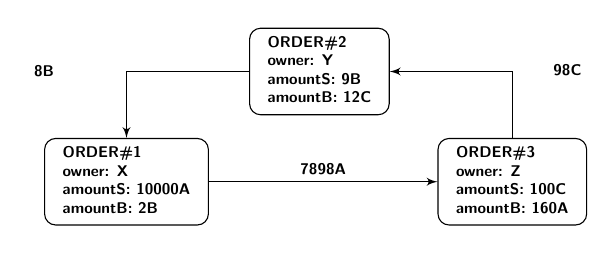
\begin{tikzpicture}[
    auto, 
    node distance=2cm,
    >=latex',
    font=\bfseries\footnotesize\sffamily,
    order/.style={
		scale=0.7,
		rectangle,
		rounded corners,
		draw=black, 
		text centered,
%		text width=5cm,
		minimum height=12mm,
		fill=white
	},
	label/.style={
		scale=0.7
	}
  ]
    % We start by placing the blocks

  \node [order] (order2) 
 {%
 \begin{tabular}{l}
  \textbf{ORDER\#2}\\
  \textbf{owner: Y}\\
  \textbf{amountS: 9B}\\
  \textbf{amountB: 12C}
 \end{tabular}
 };
 
  \node [order, below of=order2, xshift=-3.5cm] (order1) 
 {%
 \begin{tabular}{l}
  \textbf{ORDER\#1}\\
  \textbf{owner: X}\\
  \textbf{amountS: 10000A}\\
  \textbf{amountB: 2B}
 \end{tabular}
 };
 
 
  \node [order, below of=order2, xshift=3.5cm] (order3) 
 {%
 \begin{tabular}{l}
  \textbf{ORDER\#3}\\
  \textbf{owner: Z}\\
  \textbf{amountS: 100C}\\
  \textbf{amountB: 160A}
 \end{tabular}
 };
 
 \draw [draw,->] (order1) -- node [label] {\textbf{7898A}} (order3);
 \draw [draw,->] (order2) -| node [label, xshift=-1.8cm] {\textbf{8B}} (order1);
 \draw [draw,->] (order3) |- node [label, xshift=1cm, yshift=0.24cm] {\textbf{98C}} (order2);

\end{tikzpicture}

\caption{An order-ring of 3 orders}
\label{fig:ring}
\end{figurehere}
\end{center}


The above figure shows an order-ring of 3 orders. Each order's token to sell (\verb|tokenS|) is another order's token to buy (\verb|tokenB|). It creates a loop that allows each order to exchange their desired tokens without requiring an opposing order for its pair. Traditional order pair trades can, of course, still be executed, in what is essentially a special case of an order-ring. 

上面的图片显示了一个包含了三个订单的环路订单。每一个订单中希望卖出的代币是另外一个订单中希望买到的代币。它创建了一个环路,允许每一个订单交易他们需要的代币,但并不需要相应交易对的对手单。当然,传统的订单对交易仍然可以执行,本质上是一个特殊的环路订单。


\begin{definition}[订单环路] Let $C_{0}$, $C_{1}$, $\cdots$, $C_{n-1}$ be $n$ different tokens, $O_{0\rightarrow 1}$, $\cdots$, $O_{i\rightarrow i\oplus 1}$, $\cdots$, $O_{n-1 \rightarrow 0}$ be $n$ orders. Those orders can form a order-ring for trading:
$$O_{0\rightarrow 1} \rightarrow \cdots \rightarrow O_{i\rightarrow i\oplus 1} \rightarrow \cdots \rightarrow O_{n-1\rightarrow 0} \text{, }$$
where $n$ is the length of the order-ring, and $i\oplus 1 \equiv i+1 \mod n$.
\end{definition}

 C0, C1,… ,Cn-1是n个不同的代币,O0→1, …, Oi→i⊕1, …, On-1→0是n个订单。这些订单形成了用于交易的订单环路: 
O0→1, …, Oi→i⊕1, …, On-1→0
n是环路订单的长度。i⊕1≡i + 1。


An order-ring is valid when all component transactions can be executed at an exchange rate equal to or better than the original rate specified implicitly by the user. To verify order-ring validity, Loopring protocol smart contracts must receive order-rings from ring-miners where the product of the original exchange rates of all orders is equal to or greater than 1.

当一个环路订单中所有的交易元素都可以以用户自己定义的原始汇率或者以优于用户自己定义的原始汇率执行时,那么这个环路订单是有效的。为了验证环路订单的有效性,路印协议智能合约必须接收来自于环路矿工的环路订单,要求所有订单的原始交易汇率大于或者等于1。


Let's assume Alice and Bob want to trade their token \verb|A| and \verb|B|. Alice has 15 token \verb|A| and she wants 4 token \verb|B| for them; Bob has 10 token \verb|B|  and he wants 30 token \verb|A| for them.

我们假设爱丽丝和鲍勃希望交易代币A与代币B。爱丽丝持有15个代币A,希望将15个代币A交换为4个代币B;鲍勃持有10个代币B,希望将10个代币B交换为30个代币A。


Who is buying and who is selling? This depends only on the asset we fix to give price quotations. If token \verb|A| is the reference, then Alice is buying token \verb|B| for the price of ${15 \over 4} = 3.75$\verb|A|, while Bob is selling 10 token \verb|B| for the price of ${30 \over 10} = 3.00$\verb|A|. In the case of fixing token \verb|B| as reference, we say that Alice is selling 15 token \verb|A| for the price of ${4\over 15}=0.26666667$\verb|B| and Bob is buying 10 token \verb|A| for the price of ${10 \over 30}=0.33333334$\verb|B|. Hence, who's the buyer or seller is arbitrary.

那么谁是买家谁是卖家呢?这只取决于我们提供报价的资产。如果以代币A作为参照,那么爱丽丝作为买家,以1B=3.75A的价格买入。同时鲍勃作为卖家,以1B=3A价格卖出。在以代币B作为参照的例子中,爱丽丝作为卖家,以1A=0.26666667B的价格卖出,鲍勃作为买家,以1A=0.33333337B的价格买入。因此,同一个交易者既可以是买方也可以是卖方。


In the first situation Alice is willing to pay a higher price ($3.75$\verb|A|) than the price Bob is selling his tokens for ($3.00$\verb|A|), while in the second situation Bob is willing to pay a higher price ($0.33333334$\verb|B|) than the price Alice is selling her tokens for ($0.26666667$\verb|B|). It is clear that a trade is possible whenever the buyer is willing to pay an equal or higher price than the seller's price.

第一种情形,爱丽丝愿意支付的价格(1B=3.75A)高于鲍勃希望卖出的价格(1B=3A);第二种情形,鲍勃愿意支付的价格(1A=0.33333337B)高于爱丽丝希望卖出的价格(1A=0.26666667B)。很明显,只有买家愿意支付的价格大于或者等于卖家卖出的价格时,交易才有可能实现。


\begin{equation}
{{15\over 4} \over {30\over 10}} = {{10\over 30} \over {4\over 15}}={15 \over 4} \cdot {10 \over 30} = 1.25 > 1
\end{equation}

Thus, for a set of $n$ orders to be able to be filled, fully or partially, we need to know if the product of each one of the exchange rates as buy orders results in a number greater or equal to 1. If so, all the $n$ orders can be either partially, or totally filled \cite{supersymmetry}.

因此,一组n个订单想要部分或者全部成交,我们需要知道以每一个产品作为买家来计算的数值是否大于或者等于1。如果大于或者等于1,那么所有的n个订单可以部分或者全部成交[17]。


If we introduce a third counterparty, Charlie, such that  Alice wants to give $x_1$ token \verb|A| and receive $y_1$ token \verb|B|, Bob wants to give $x_2$ token \verb|B| and receive $y_2$ token \verb|C|, and Charlie wants to give $x_3$ token \verb|C| and receive $y_3$ token \verb|A|. The necessary tokens are present, and the trade is possible if:

 如果我们引入第三个交易对手查理,爱丽丝希望以x1价格卖出代币A, 以y1价格买入代币B。鲍勃希望以x2价格卖出代币B,以y2价格买入代币C,查理希望以x3价格卖出代币C,以y3价格买入代币A。那么该交易成交需要满足下面的关系式:


\begin{equation}
{{x1 \cdot x_2 \cdot x_3 \over y_1 \cdot y_2 \cdot y_3} \geq 1}
\end{equation}


See section \ref{anatomy} for more details about Loopring's orders.

关于路印订单在7.1章节会做详细阐述。


\section{生态系统的参与者\label{sec:ecosystem}}
The following ecosystem participants jointly provide all functionalities a centralized exchange has to offer. 

下述生态系统参与者共同提供中心化交易所的所有功能。

\begin{itemize}

\item \textbf{Wallets}: A common wallet service or interface that gives users access to their tokens and a way to send orders to the Loopring network. Wallets will be incentivized to produce orders by sharing fees with ring-miners (see section \ref{sec:token}). With the belief that the future of trading will take place within the safety of individual user's wallets, connecting these liquidity pools through our protocol is paramount.

钱包:一个普通的钱包服务或接口,让用户可以访问他们的代币并且可以发送订单到路印网络。通过与环路矿工共享费用,钱包将会受到激励产生订单(见第8节)。我们坚信,未来的交易将会发生在安全的用户个人钱包内,所以通过路印协议连接这些流动的资金池是至关重要的


\item \textbf{Consortium Liquidity Sharing Blockchain/Relay-Mesh}: A relay-mesh network for order \& liquidity sharing. When nodes run Loopring relay software, they are able to join an existing network and share liquidity with other relays over a consortium blockchain. The consortium blockchain we are building as a first implementation has near real time order sharing (1-2 second blocks), and trims old history to allow for faster download by new nodes. Notably, relays need not join this consortium; they can act alone and not share liquidity with others, or, they can start and manage their own liquidity sharing network.

联盟流动性共享区块链/中继网格:一种用于订单与流动性共享的中继网络。当节点运行路印中继软件时,节点有能力加入一个已经存在的网络并且通过联盟区块链与其他中继共享流动性。我们正在构建的并且是第一个实现的联盟区块链可以做到实时共享订单,梳理历史交允许新的节点更快速的下载。值得注意的是,中继并不需要加入这个联盟;他们可以独立工作不与其他中继共享流动性,或者他们可以创建并且管理自己的流动性共享网络。


\item \textbf{Relays/Ring-Miners}: Relays are nodes that receive orders from wallets or the relay-mesh, maintain public order books and trade history, and optionally broadcast orders to other relays (via any arbitrary off-chain medium) and/or relay-mesh nodes. Ring-mining is a feature -- not a requirement -- of relays. It is computationally heavy and is done completely off-chain. We call relays with the ring-mining feature turned on \enquote{Ring-Miners}, who produce order-rings by stitching together disparate orders. Relays are free in (1) how they choose to communicate with one another, (2) how they build their order books, and (3) how they mine order-rings (mining algorithms).

中继/环路矿工:中继就是从钱包或者中继网格接收订单的节点,维护公共订单帐簿,选择性的广播订单到其他中继或者中继网格节点。环路挖矿是是中继的一个特点,但并不是必须的。他的计算量很大,计算在线下完成。我们将具有环路挖矿功能的中继称为环路矿工,环路矿工通过拼接不同的订单产生环路订单。中继的以下操作是自由的(1)中继之间的相互通信(2)中继如何建立订单簿(3)中继如何进行环路挖矿。


\item \textbf{Loopring Protocol Smart Contracts (LPSC)}: A set of public and free smart contracts that checks order-rings received from ring-miners, trustlessly settles and transfers tokens on behalf of users, incentivizes ring-miners and wallets with fees, and emits events. Relays/order browsers listen to these events to keep their order books and trade history up to date. See appendix \ref{app:protocol_ethereum} for details.

路印协议智能合约LPSC:指的是一系列公开并且免费的智能合约,用于核实来自于环路矿工的环路订单。站在用户的立场无需信任的传输和交易代币,通过费用激励环路矿工与钱包,发起交易事件。中继浏览器与订单浏览器收听这些事件,以保证实时更新他们的订单簿与交易历史。详细请参考附录A


\item \textbf{Asset Tokenization Services (ATS)}: A bridge between assets that cannot be directly traded on Loopring. They are centralized services run by trustworthy companies or organizations. Users deposit assets (real, fiat or tokens from other chains) and get tokens issued, which can be redeemed for the deposit in the future. Loopring is not a cross-chain exchange protocol (until a suitable solution exists), but ATS enable trading of ERC20 tokens \cite{ERC20} with physical assets as well as assets on other blockchains. 

资产标记服务ATS:为不能直接在路印协议上交易的资产架起了桥梁。可以信任的公司或者组织为他们提供中心化的服务。用户存入资产(可以是真实的、扁平的资产或是来自其他链的代币),然后签发代币,以供将来赎回资产使用。路印协议并不是一个跨链交易协议(除非已经有何合适的跨链解决方案)。但是资产标记服务使得ERC2.0代币可以与实物资产交易,也可以与其他链上的资产交易。


\end{itemize}


\section{交易过程\label{sec:process}}



\begin{enumerate} 


\item \textbf{Protocol Authorization}: In figure \ref{fig:process}, user \verb|Y| who wants to exchange tokens authorizes the LPSC to handle \verb|amountS| of token \verb|B| the user wants to sell. This does not lock the user's tokens, who remains free to move them while the order is processed.

协议授权:如图二所示,用户Y将代币的买卖需求授权给路印协议智能合约,路印协议智能合约代替用户寻找合适的代币B卖家并完成代币交易。这一过程并不会锁定用户的代币,在订单处理过程中用户仍然可以自由支配他们的代币。


\item \textbf{Order Creation}: The current rate and order book for token \verb|B| vs token \verb|C|, are provided by relays or other agents hooked up to the network, such as order book browsers. User \verb|Y| places an order (limit order) specifying \verb|amountS| and \verb|amountB| and other parameters through any integrated wallet interface. An amount of LRx can be added to the order as a fee for ring-miners; higher LRx fee means a better chance to be processed earlier by ring-miners. The order's hash is signed with user \verb|Y|'s private-key.

创建订单:代币B与代币C的当前汇率与订单簿是由中继或者其他连接到网络的机构提供,比如订单簿浏览器。用户Y通过任意的集成钱包接口提交了订单,明确了买卖代币的数量以及其他参数。在订单中放置一定数量的LRx作为支付给环路矿工的费用;矿工会优先处理支付矿工费较高的订单。订单的哈希值将会使用用户Y的私钥进行数字签名。


\item \textbf{Order Broadcast}: The wallet sends the order and its signature to one or more relays. Relays update their public order book. The protocol doesn't require order books to be built in a certain way, such as first-come-first-serve. Instead, relays have the power to make their own design decisions in building their order books.

订单广播:钱包将订单与数字签名发送给一个或多个中继。中继更新他们的公共订单簿。该协议不需要以某种特定的方式创建订单,比如先到先服务。恰恰相反,中继有能力自己做好设计决策创建订单簿。


\item \textbf{Liquidity Sharing}: Relays broadcast the order to other relays through any arbitrary communication medium. Once again, there is flexibility how/whether nodes interact. To facilitate a certain level of network connectivity, there is a built-in liquidity sharing relay-mesh using a consortium blockchain. As mentioned in the prior section, this relay-mesh is optimized for speed and inclusivity.

流动性共享:中继通过任意的通信媒介将订单广播给其他中继。再次,节点之间是否相互作用以及如何相互影响很具有灵活性。为了增强网络的连接能力,通过联盟区块链设置了一个内建的流动性共享中继网格。正如前面章节所提到的,这个中继网格在速度与兼容性方面做了优化。


\begin{center}
\begin{figurehere}
\centering
\tikzstyle{block} = [draw, fill=blue!20, rectangle, 
    minimum height=3em, minimum width=6em]
\tikzstyle{sum} = [draw, fill=blue!20, circle, node distance=1cm]
\tikzstyle{input} = [coordinate]
\tikzstyle{output} = [coordinate]
\tikzstyle{pinstyle} = [pin edge={to-,thin,black}]

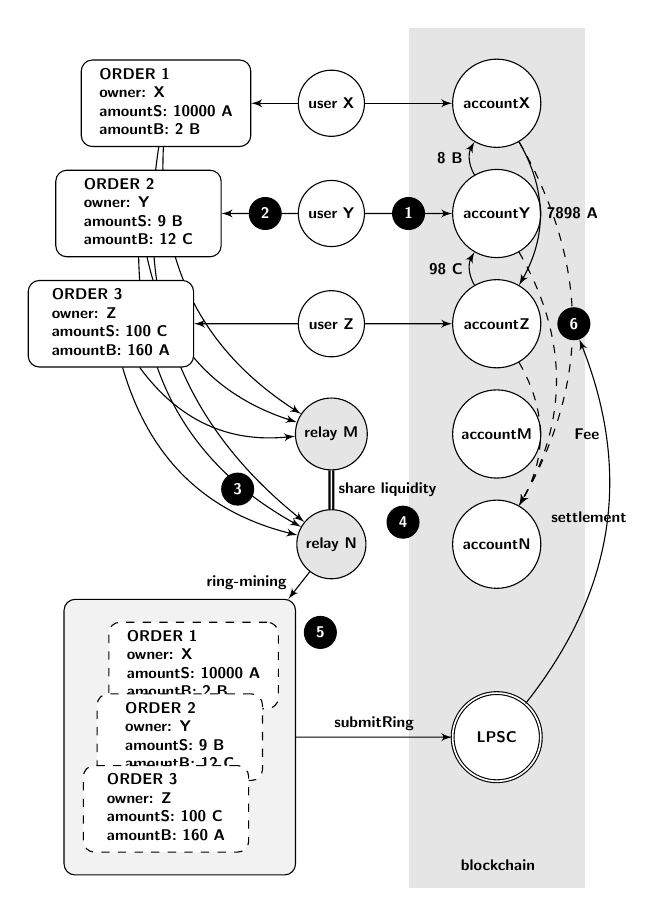
\begin{tikzpicture}[
    auto, 
    scale=0.7,
    node distance=2cm,
    >=latex',
    font=\bfseries\footnotesize\sffamily,
    order/.style={
		rectangle,
		scale=0.7,
		rounded corners,
		draw=black, 
		text centered,
%		text width=5cm,
		minimum height=12mm,
		minimum width=30mm,
		fill=white
	},
	role/.style={
		circle,
		scale=0.7,
		draw=black, 
		text centered,
%		text width=5cm,
		minimum height=12mm,
		minimum width=12mm,
		fill=white
	},
	steps/.style={
		circle,
		scale=0.7,
		draw=black, 
		text centered,
%		text width=5cm,
%		minimum height=12mm,
%		minimum width=12mm,
		fill=black,
		text=white
	},
	account/.style={
		circle,
		scale=0.7,
		draw=black, 
		text centered,
%		text width=5cm,
		minimum height=16mm,
		minimum width=16mm,
		fill=white
	},
	label/.style={
	  scale=0.7
    }
  ]

 
 \node [role] (user1)  {user X};
 \node [role, below of=user1] (user2)  {user Y};
 \node [role, below of=user2] (user3)  {user Z};
 \node [role, below of=user3, fill=gray!20] (relay1)  {relay M};
 \node [role, below of=relay1, fill=gray!20] (relay2)  {relay N};

 
 \node [order, left of=user1, xshift=-1cm] (order1) 
 {%
 \begin{tabular}{l}
  \textbf{ORDER 1}\\
  \textbf{owner: X}\\
  \textbf{amountS: 10000 A}\\
  \textbf{amountB: 2 B}
 \end{tabular}
 };
 
 \draw [draw, ->]  (user1) -- (order1) [label]{};
 \draw [bend right,->] (order1) to node [auto, scale=0.7] {} (relay1);
 \draw [bend right,->] (order1) to node [auto, scale=0.7] {} (relay2);
% \draw [draw, ->]  (order1) |- (relay1) [label]{};
% \draw [draw, ->]  (order1) |- (relay2) [label]{};
 
 \node [order,left of=user2, xshift=-1.5cm] (order2) 
 {%
 \begin{tabular}{l}
  \textbf{ORDER 2}\\
  \textbf{owner: Y}\\
  \textbf{amountS: 9  B}\\
  \textbf{amountB: 12 C}
 \end{tabular}
 };
 \draw [draw, ->]  (user2) -- (order2) [label]{};
 \draw [bend right,->] (order2) to node [auto, scale=0.7] {} (relay1);
 \draw [bend right,->] (order2) to node [auto, scale=0.7] {} (relay2);
% \draw [draw, ->]  (order2) |- (relay1) [label]{};
% \draw [draw, ->]  (order2) |- (relay2) [label]{};
% 
\node [order, left of=user3, xshift=-2cm] (order3) 
 {%
 \begin{tabular}{l}
  \textbf{ORDER 3}\\
  \textbf{owner: Z}\\
  \textbf{amountS: 100 C}\\
  \textbf{amountB: 160 A}
 \end{tabular}
 };
 \draw [draw, ->]  (user3) -- (order3) [label]{};
 \draw [bend right,->] (order3) to node [auto, scale=0.7] {} (relay1);
 \draw [bend right,->] (order3) to node [auto, scale=0.7] {} (relay2);
% \draw [draw, ->]  (order3) |- (relay1) [label]{};
% \draw [draw, ->]  (order3) |- (relay2) [label]{};
 
% // The Ring
\node [order, 
yshift=-1.5cm,
xshift=-2.75cm,
below of=relay2,
fill=gray!10,
minimum width=4.2cm,
minimum height=5cm] (ring) {};


\node [order, dashed, below of=relay2,yshift=-0.2cm,xshift=-2.5cm] (order11) 
 {%
 \begin{tabular}{l}
  \textbf{ORDER 1}\\
  \textbf{owner: X}\\
  \textbf{amountS: 10000 A}\\
  \textbf{amountB: 2 B}
 \end{tabular}
 };
 \node [order, dashed,below of=order11,xshift=-0.25cm,yshift=0.7cm] (order21) 
 {%
 \begin{tabular}{l}
  \textbf{ORDER 2}\\
  \textbf{owner: Y}\\
  \textbf{amountS: 9  B}\\
  \textbf{amountB: 12 C}
 \end{tabular}
 };
\node [order, dashed,below of=order21,xshift=-0.25cm,yshift=0.7cm] (order31) 
 {%
 \begin{tabular}{l}
  \textbf{ORDER 3}\\
  \textbf{owner: Z}\\
  \textbf{amountS: 100 C}\\
  \textbf{amountB: 160 A}
 \end{tabular}
 };
 
 % // The blockchain
\node [
rectangle,
fill=gray!20, 
right of=user1,
yshift=-4.5cm,
xshift=0.1cm,
scale=0.7,
minimum width=3.2cm,
minimum height=15.6cm] (blockchain) {\parbox[b][15cm]{1.3cm}{blockchain}};
% blockchain accounts
  \node [account, right of=user1, xshift=1cm] (account1)  {accountX};
  \node [account, right of=user2, xshift=1cm] (account2)  {accountY};
  \node [account, right of=user3, xshift=1cm] (account3)  {accountZ};
  \node [account, right of=relay1, xshift=1cm] (account4)  {accountM};
  \node [account, right of=relay2, xshift=1cm] (account5)  {accountN};
  \node [account, double, below of=account5, yshift=-1.5cm] (psc)  {LPSC};
  
 \draw [draw, ->]  (user1) -- (account1) [label]{};
 \draw [draw, ->]  (user2) -- (account2) [label]{};
 \draw [draw, ->]  (user3) -- (account3) [label]{};
% \draw [draw, ->]  (relay1) -- (account4) [label]{};
% \draw [draw, ->]  (relay2) -- (account5) [label]{};
 \draw [draw, double, thick]  (relay1) to node [auto, scale=0.7] {share liquidity}  (relay2) [label]{};
% \draw [draw, ->]  (relay1) -- (ring) [label]{};
 \draw [draw, ->]  (relay2) to node [auto, scale=0.7, xshift=-1.8cm, yshift=0.3cm] {ring-mining}  (ring) [label]{};
 \draw [draw, ->]  (ring) to node [auto, scale=0.7] {submitRing} (psc) [label]{};
 
 \draw [bend left,->] (account1) to node [auto, scale=0.7] {\textbf{7898 A}} (account3);
 \draw [bend left,->] (account2) to node [auto, scale=0.7] {\textbf{8 B}} (account1);
 \draw [bend left,->] (account3) to node [auto, scale=0.7] {\textbf{98 C}} (account2);
 
 \draw [bend left,->, dashed] (account1) to node [auto, scale=0.7] {} (account5);
 \draw [bend left,->, dashed] (account2) to node [auto, scale=0.7] {} (account5);
 \draw [bend left,->, dashed] (account3) to node [auto, scale=0.7, xshift=.5cm] {\textbf{Fee}} (account5);
  
  
% \draw [draw,->] (order1) -- node [label] {\textbf{7898 A}} (order3);
% \draw [draw,->] (order2) -| node [label, xshift=-1.8cm] {\textbf{8 B}} (order1);
% \draw [draw,->] (order3) |- node [label, xshift=1cm, yshift=0.24cm] {\textbf{98 C}} (order2);

\node [steps, right of=user2, xshift=-0.6cm] () {1};
\node [steps, left of=user2, xshift=0.8cm] () {2};
\node [steps, left of=relay2, xshift=0.3cm, yshift=1cm] () {3};
\node [steps, left of=relay1, xshift=3.3cm, yshift=-1.6cm] () {4};
\node [steps, below of=relay2, xshift=-0.2cm, yshift=0.4cm] () {5};
\node [steps, right of=account3, xshift=-0.6cm] (step5) {6};

 \draw [bend right, ->]  (psc) to node [auto, scale=0.7, xshift=0.5cm] {settlement} (step5) [label]{};
 
\end{tikzpicture}

\caption{Loopring Exchange Process}
\label{fig:process}
\end{figurehere}
\end{center}



\item \textbf{Ring-Mining (Order Matching)}:  Ring-miners try to fill the order fully or partially at the given exchange rate or better by matching it with multiple other orders. Ring-mining is the main reason why the protocol is able to provide high liquidity over any pair. If the executed rate is better than what user Y specified, margin is shared amongst all orders in the order-ring. As a reward, the ring-miner chooses between claiming part of the margin (Margin-Split, and giving back the LRx to the user), or simply keeping the LRx fee.

环路挖矿(订单挖矿):环路挖矿矿工尝试按照给定的汇率或者优于给定的汇率进行多个订单匹配,以期完成全部或者部分订单交易。环路挖矿是协议有能力提供超出任何交易对高流动性的主要原因。如果执行汇率优于用户Y指定的汇率,那么边缘利润将会在环路订单中的所有订单共享。作为奖励,环路矿工可以选择拥有边缘利润的一部分(边缘利润进行分割,部分LRx返还给用户),也可以选择直接持有LRx作为矿工费用。


\item \textbf{Verification \& Settlement}: The order-ring is received by LPSC. It makes multiple checks to verify the ring-miner supplied data and determines if the order-ring can be settled fully or partially (depending on the fill rate of orders in-ring and tokens in users' wallets). If all checks are successful, the contract atomically transfers the tokens to users and pays the ring-miner and wallet fees at the same time. If user \verb|Y|'s balance as determined by the LPSC is insufficient, it will be considered scaled-down: a scaled-down order will automatically scale up to its original size if sufficient funds are deposited to its address, unlike a cancellation, which is a one way manual operation and cannot be reversed.

审核与结算:通过路印协议智能合约收到环路订单。它会进行多重审核以验证环路矿工提供的数据与决策,环路订单是否能全部成交或者部分成交取决于环路订单中的汇率以及用户钱包里的代币。如果所有的审核成功通过,智能合约自动发送代币给用户,同时支付相应的费用给环路矿工以及钱包。如果路印协议智能合约判定用户Y的资产数量不足,订单的规模将会被缩小。如果有足够的资金存入相应的地址,这个被缩小规模的订单会自动放大规模至原始订单大小,这不同于取消订单操作,取消订单是一种单向的手动操作而且是不可逆转的。



\end{enumerate}





%
%\end{multicols}
%
%\begin{center}
%\begin{figurehere}
%\includegraphics[height=8cm]{images/en_protocol.png}
%\caption{Loopring Trading Process}
%\label{fig: Loopringrotocol}
%\end{figurehere}
%\end{center}
%
%\begin{multicols}{2}

\section{运营的灵活性\label{sec:business_model}}
It's important to note that Loopring's open standard allows participants significant flexibility in how they operate. Actors are free to implement novel business models and provide value for users, earning LRx fees on volume or other metrics in the process (if they so choose). The ecosystem is modular and meant to support participation from a multitude of applications.

值得注意的是,路印协议的开放标准给予参与者很大的操作灵活性。参与者可以自由的执行新颖的商业模型同时为用户提供价值,在此过程中按照交易量或者其他的指标赚取LRx费用。整个生态系统是模块化的,旨在为参与者众多的应用提供支持。


\subsection{订单簿\label{sec:order_book}}
Relays can design their order books in any number of ways to display and match users' orders. A first implementation of our own order book follows an OTC model, where limit orders are positioned based on price alone. Timestamps of orders, in other words, have no bearing on the order book. However, a relay is free to design their order book in such a way as to emulate a typical centralized exchange's matching engine, where orders are ranked by price, while respecting timestamps as well. If a relay was inclined to offer this type of order book, they can own/integrate with a wallet, and have those wallet orders sent solely to the single relay, who would then be able to match orders based on time. Any such configuration is possible.


中继可以以多种方式设计自己的订单簿,以显示和匹配用户的订单。我们订单簿的第一次执行遵循OTC模型,此时限价单是基于价格单独定位的。换句话说,订单的时间戳与订单簿没有关系。然而,中继可以自由的设计他们的订单簿,目的是为了达到一个典型的中心化交易所的订单匹配引擎的能力,中心化交易引擎将订单按价格排序同时也尊重时间戳。 如果中继倾向于提供这种类型的订单簿,那么他们可以拥有钱包,同时仅仅将这些钱包订单发送给单一的中继,这个中继就可以按照时间来匹配订单。任意的这样的配置是可能实现的。

Whereas other DEX protocols at times require Relays to have resources - initial token balances to place taker orders - Loopring Relays need only find matchable orders to consummate a trade, and can do so without initial tokens.

然而,其他的去中心化的协议需要中继以便获得资源(提交订单需要的初始代币余额)。而路印中继不需要初始代币,仅仅需要寻找匹配的订单来完成交易。

\subsection{流动性共享\label{sec:liquidity_sharing}}
Relays are free to design how they share liquidity (orders) with each other. Our consortium blockchain is but one solution to accomplish this, and the ecosystem is free to network and communicate as they wish. Besides joining a consortium blockchain, they can build and manage their own, creating rules/incentives as they see fit. Relays can also work alone, as seen in the time-sensitive wallet implementation. Of course, there are clear advantages in communicating with other Relays in pursuit of network effects, however, different business models could merit peculiar sharing designs and split fees in any number of ways.

中继可以自由设计如何与其他中继共享订单。我们的联盟区块链就是一种解决方案,同时这个生态系统对网络是免费的,他们之间可以自由通信。除了加入联盟区块链,中继可以创建他们认为合适的规则和激励机制。中继也可以单独工作,正如在时间敏感钱包运行时所见到的。当然,在追求网络效应方面,中继之间的通讯也具有明显的优势。然而,不同的商业模式可以采用特殊的共享设计,并以多种方式分担费用。


\section{协议规范\label{sec:protocol}}

\subsection{Anatomy of an Order\label{anatomy}}
An order is a pack of data that describes the intent of the user's trade. A Loopring order is defined using the Uni-Directional Order Model, or UDOM, as follows:

一个订单就是一组描述了用户交易目的的数据。路印订单采用了如下所述的单向顺序模型或者UDOM模型。


\begin{verbatim}
  message Order {
    address protocol;
    address owner;
    address tokenS;
    address tokenB;
    uint256 amountS;
    uint256 amountB;
    unit256 lrcFee
    unit256 validSince; // Seconds since epoch
    unit256 validUntil; // Seconds since epoch
    uint8   marginSplitPercentage;  // [1-100]
    bool    buyNoMoreThanAmountB;
    uint256 walletId;
    // Dual-Authoring address
    address authAddr;
   	// v, r, s are parts of the signature
    uint8   v;       
    bytes32 r;
    bytes32 s;
    // Dual-Authoring private-key,
    // not used for calculating order's hash,
    // thus it is NOT signed.
    string  authKey;          
  }
\end{verbatim}


To ensure the origin of the order, it is signed against the hash of its parameters, excluding \verb|authAddr|, with the user's private-key. The \verb|authAddr| parameter is used for signing  order-rings that this order is part of, which prevents front-running. Please reference section \ref{sec:dual_authoring} for more details. The signature is represented by the \verb|v|, \verb|r|, and \verb|s| fields, and is sent alongside the order parameters over the network. This guarantees the order stays immutable during its whole lifetime. Even though the order never changes, the protocol can still compute its current state based on the balance of its address along with other variables.

为了确保原始订单,使用用户的私钥对散列参数(不包括授权地址)进行数字签名。授权地址参数用于环路订单签名,用于防止抢先交易。更详细的介绍请参考9.1章节。签名用v,r与s字段表示,可以与订单参数一起发布到网络上。这就保证了订单在整个过程中保持不变。即使订单不会改变,协议仍然可以根据资产余额与其他变量计算订单当前状态。



UDOM doesn't include a price (which must be a floating-point number by nature), but, instead uses the term \verb|rate| or $r$, which is expressed as \verb|amountS|/\verb|amountB|. The rate is not a floating-point number but an expression that will only be evaluated with other unsigned integers on demand, to keep all intermediate results as unsigned integers and increase calculation accuracy. 

UDOM模型不包括价格(价格必须是一个浮点数),并不使用汇率等词汇,而是使用了amontS/amontB来表述。这个比例并不是一个浮点数,而是按照需要与其他无符号整数一起计算以保持所有的中间结果。

\subsubsection{买入数量}

When a ring-miner ring-matches orders, it's possible that a better rate will be executable, allowing users to get more \verb|tokenB| than the \verb|amountB| they specified. However, if \verb|buyNoMoreThanAmountB| is set to \verb|True|, the protocol ensures users receive no more than \verb|amountB| of \verb|tokenB|. Thus, UDOM's \verb|buyNoMoreThantokenB| parameter determines when an order is considered completely filled. \verb|buyNoMoreThantokenB| applies a cap on either \verb|amountS| or \verb|amountB|, and allows users to express more granular trade intentions than traditional buy/sell orders.

当环路矿工进行环路订单匹配时,有可能会选择一个更合适的汇率进行交易,这样就有可能使用户得到比他们自己指定的数量更多的代币。然而,如果设置购买数量不超过AmountB,协议会保证用户收到的代币B数量不超过AmountB。因此,UDOM模型中决定购买不超过一定数量代币B的参数决定了一个订单在何时全部完成。可以为需要买卖代币的数量amountB与amountS设置上限,相比于传统买卖订单,这样就允许用户表达出更多的代币购买意向。



For example: with \verb|amountS| = 10 and \verb|amountB| = 2, the rate $r$ = 10/2 = 5. Thus the user is willing to sell 5 \verb|tokenS| for each \verb|tokenB|. The ring-miner matches and finds the user a rate of 4, allowing the user to receive 2.5 \verb|tokenB| instead of 2. However, if the user only wants 2 \verb|tokenB| and set the \verb|buyNoMoreThanAmountB| flag to \verb|True|, the LPSC performs the transaction at a rate of 4 and the user sells 4 \verb|tokenS| for each \verb|tokenB|, effectively saving 2 \verb|tokenS|. Keep in mind this does not take into account mining fees (See section \ref{sec:fee_model}).

例如:卖出数量=10,买入数量=2,汇率r=10/2=5。因此用户愿意用5个代币S换取1个代币B。环路矿工匹配订单为用户找到了更加合适的汇率r=4,这样用户最终会收到2.5个代币B而不是2个。然而,如果用户只想得到2个代币B,并且将标签“用户只想得到2个代币B”设置为真值,路印协议智能合约将会按照汇率r=4执行代币交易,用户使用4个代币S换取1个代币B,这样就为用户有效的节省了2个代币S。请记住,这里并没有考虑矿工费用。


Indeed, if we use


\begin{verbatim}
	      Order(amountS,tokenS,
	            amountB,tokenB,
	            buyNoMoreThantokenB)
\end{verbatim}

to represent an order in a simplified form, then for ETH/USD markets on a traditional exchange, traditional buy-sell modeling can express the 1st and the 3rd order below, but not the other two:


实际上,如果我们使用下述简单的表达式代表一个订单,对于传统交易所的ETH/USD交易市场,传统的交易模型只能表达下述的第一与第三个订单,而不能表达其他两个订单:



\begin{enumerate}
	\item Sell 10 ETH at price of 300 USD/ETH. This order can expressed as: \verb|Order(10, ETH, 3000, USD, False)|.
	\item 以300USD/ETH的价格卖出10个ETH。这个订单可以表为:Order(10,ETH,3000,USD,False)

	\item Sell ETH at price of 300 USD/ETH to get 3000 USD. This order can expressed as: \verb|Order(10, ETH, 3000, USD, True)|.
	\item 以300USD/ETH的价格卖出ETH以得到3000USD。这个订单可以表达为:Order(10,ETH,3000,USD,True)

	\item Buy 10 ETH at price of 300 USD/ETH, This order can expressed as: \verb|Order(3000, USD, 10, ETH, True)|.
	\item 以300USD/ETH的价格买入10个ETH。这个订单可以表为:Order(3000,USD,10,ETH,True)

	\item Spend 3000 USD to buy as many ETH as possible at price of 300 USD/ETH, This order can expressed as: \verb|Order(3000, USD, 10, ETH, False)|.
	\item 花费3000USD以300USD/ETH的价格,尽可能多的购买ETH。这个订单可以表为:Order(3000,USD,10,ETH,False)

\end{enumerate}



\subsection{环路验证\label{sec:ring_verification}}

The Loopring Smart Contracts do not perform exchange rate or amount calculations, but must receive and verify what the ring-miners supply for these values. These calculations are done by ring-miners for two main reasons: (1) the programming language for smart contracts, such as solidity\cite{dannen2017introducing} on Ethereum, does not have support for floating point math, especially $pow(x, 1/n)$ (calculating the n-th root of a floating point number), and (2) it is desirable for the computation to be made off-chain to reduce blockchain computation and cost.

路印协议智能合约不进行交易汇率和交易数量的计算,但是必须验证环路矿工提供的数据。交易汇率与交易数量的计算由环路矿工完成,主要是基于以下两个原因:(1)智能合约编程语言不支持浮点运算,如以太坊网络的solidify语言[19]。尤其是工作量证明机制(x; 1/n),需要计算一个浮点数的n次方根。(2)链下计算是可取的,因为链下计算可以减小区块链的计算量与成本。


\subsubsection{子环路检查\label{sec:sub_ring_check}}
This step prevents arbitrageurs from unfairly realizing all the margin in an order-ring by implementing new orders within it. Essentially, once a valid order-ring is found by a ring-miner, it could be tempting to add other orders to the order-ring to fully absorb the users' margin (rate discounts). As illustrated by figure \ref{fig:subring} below, carefully calculated $x1$, $y1$, $x2$ and $y2$ will make the product of all orders' rate be exactly 1 so there will be no rate discount. 

这一步可以防止套利者通过在环路订单中执行新的订单占据环路订单中的所有边缘利润,至关重要的是,一旦环路矿工发现一个有效的环路订单,它会试图这向这个环路订单中增加其他订单,全部吸收用户的边缘利润。如图三所表示,详细计算x1,y1,x2与y2会使得所有订单的汇率精准的等于1,因此就不存在汇率折扣。


\begin{center}
\begin{figurehere}
\centering
\tikzstyle{block} = [draw, fill=blue!20, rectangle, 
    minimum height=3em, minimum width=6em]
\tikzstyle{sum} = [draw, fill=blue!20, circle, node distance=1cm]
\tikzstyle{input} = [coordinate]
\tikzstyle{output} = [coordinate]
\tikzstyle{pinstyle} = [pin edge={to-,thin,black}]

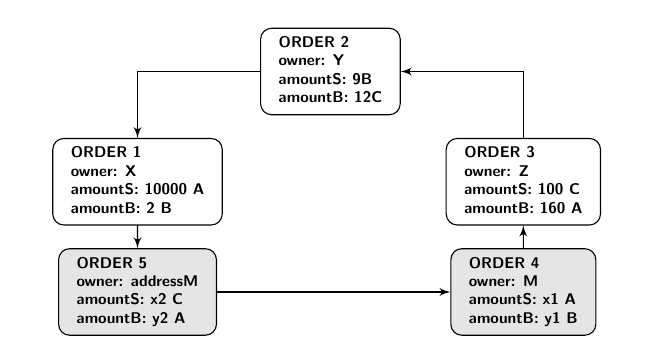
\begin{tikzpicture}[
    auto, 
    node distance=2cm,
    >=latex',
    font=\bfseries\footnotesize\sffamily,
    order/.style={
		scale=0.7,
		rectangle,
		rounded corners,
		draw=black, 
		text centered,
%		text width=5cm,
		minimum height=12mm,
		fill=white
	},
	label/.style={
		scale=0.7
	}
  ]
    % We start by placing the blocks

  \node [order] (order2) 
 {%
 \begin{tabular}{l}
  \textbf{ORDER 2}\\
  \textbf{owner: Y}\\
  \textbf{amountS: 9B}\\
  \textbf{amountB: 12C}
 \end{tabular}
 };
 
  \node [order, below of=order2, xshift=-3.5cm] (order1) 
 {%
 \begin{tabular}{l}
  \textbf{ORDER 1}\\
  \textbf{owner: X}\\
  \textbf{amountS: 10000 A}\\
  \textbf{amountB: 2 B}
 \end{tabular}
 };
 
 
  \node [order, below of=order2, xshift=3.5cm] (order3) 
 {%
 \begin{tabular}{l}
  \textbf{ORDER 3}\\
  \textbf{owner: Z}\\
  \textbf{amountS: 100 C}\\
  \textbf{amountB: 160 A}
 \end{tabular}
 };
 
   \node [order, below of=order3, fill=gray!20] (order4) 
 {%
 \begin{tabular}{l}
  \textbf{ORDER 4}\\
  \textbf{owner: M}\\
  \textbf{amountS: x1 A}\\
  \textbf{amountB: y1 B}
 \end{tabular}
 };
 
 
  \node [order, below of=order1, fill=gray!20] (order5) 
 {%
 \begin{tabular}{l}
  \textbf{ORDER 5}\\
  \textbf{owner: addressM}\\
  \textbf{amountS: x2 C}\\
  \textbf{amountB: y2 A}
 \end{tabular}
 };
 
 \draw [draw,->] (order1) -- node [label, xshift=-2cm] {} (order5);
 \draw [draw,->] (order2) -| node [label, xshift=-1.6cm] {} (order1);
 \draw [draw,->] (order3) |- node [label, xshift=1cm] {} (order2);
 \draw [draw,->] (order4) -- node [label, xshift=1.8cm] {} (order3);
 \draw [draw,->] (order5) -- node [label, yshift=0.2cm] {} (order4);
  
\end{tikzpicture}

\caption{An order-ring with sub-ring}
\label{fig:subring}
\end{figurehere}
\end{center}

This is zero-risk, zero-value add to the network, and is considered unfair conduct by the ring-miner. To prevent this, Loopring requires that a valid loop cannot contain any sub-rings. To check this, the LPSC ensures a token cannot be in a buy or sell position twice. In the above diagram, we can see that token \verb|A| is a sell token twice and a buy token twice, which would be disallowed. 

在网络中添加零值是零风险的,但是被认为是环路矿工主导的不公平行为。为了防止这类事件的发生,路印需要一个不包含任何次环的验证环路。为了确保这一点,路印协议智能合约确保同一个代币不会在买或者卖的位置出现两次。在上图中,我们看到代币A分别被买卖了两次,这一点是不允许的。


\subsubsection{汇率核实\label{sec:fill_rate_check}}


The exchange rate calculations in the order-ring are made by ring-miners for reasons stated above. It is the LPSC that must verify they're correct. First, it verifies that the buy rate the ring-miner can execute for each order is equal to or less than the original buy rate set by the user. This ensures the user gets at least the exchange rate they asked for or better on the transaction. Once the exchange rates are confirmed, the LPSC ensures that each order in the order-ring shares the same rate discount. For instance, if the discounted rate is $\gamma$, then the price for each order will be:

基于上面所陈述的原因,环路订单中的汇率计算是由环路矿工完成的。必须通过路印协议智能合约对汇率进行验证。首先,它要验证环路矿工能够执行的买入汇率等于或者小于用户设定的原始买入汇率。保证在交易过程中用户得到自己要求的汇率或者更优的汇率。汇率被确定以后,路印协议智能合约保证环路订单中的每一个订单分享同样的汇率折扣。举例说明,如果汇率折扣=γ,那么每一个订单的价格是:


$r_{0\rightarrow 1} \cdot (1-\gamma)$, $r_{1\rightarrow 2} \cdot (1-\gamma)$, $r_{2 \rightarrow 0} \cdot (1-\gamma)$, and satisfy: 

并且满足下式:



\begin{equation}
r_{0\rightarrow 1} \cdot (1-\gamma)\cdot r_{1\rightarrow 2} \cdot (1-\gamma) \cdot r_{2 \rightarrow 0} \cdot (1-\gamma) = 1
\end{equation}
hence: 

因此:



\begin{equation}
\gamma = 1- \frac{1}{\sqrt[3]{r_{0\rightarrow 1} \cdot r_{1\rightarrow 2} \cdot r_{2\rightarrow 0}}}\text{.}
\end{equation}
If the transaction crosses $n$ orders, the \texttt{discount} is: 

如果交易包含了n个订单,那么折扣是:


\begin{equation}
\gamma = 1- \frac{1}{\sqrt[n]{\prod_{i=0}^{n-1} r^i}} \text{,}
\end{equation}

where $r^i$ is the order turnover rate of $i$-th order. Obviously, only when the discount rate is $\gamma \ge 0$, can these orders be filled; and the $i$-th order ($O^i$)'s actual exchange rate is $\hat{r^i} = r^i \cdot (1-\gamma)$, $\hat{r^i}\le r^i$.

ri是i阶订单的周转率。很明显,只有当折扣率γ≥0时,这些订单才能够完成。I阶订单的实际汇率为:


Recall our prior example where Alice has 15 token \verb|A| and wants 4 token \verb|B| for them, Bob has 10 token \verb|B| and wants 30 token \verb|A| for them. If token \verb|A| is the reference, then Alice is buying token \verb|B| for $\frac{15}{4}$ = 3.75\verb|A|, while Bob is selling token \verb|B| for $\frac{30}{10}$ = 3.00\verb|A|. To calculate the discount: $\frac{150}{120}$ = 1.25 thus $\frac{1}{1.25}$ = 0.8 = $(1 −- \gamma)^2$. Thus the exchange rate that renders the trade equitable for both parties is $\sqrt{0.8}$ $\cdot$ 3.75 $\approx$ 3.3541 token \verb|A| per token \verb|B|.

Bob gives 4 token \verb|B| and receives 13.4164 token \verb|A|, more than the 12 he was expecting for those 4 tokens. Alice receives 4 token \verb|B| as intended but gives only 13.4164 token \verb|A| in exchange, less than the 15 she was willing to give for those 4 tokens.
Note, a portion of this margin will go towards paying fees to incentivize miners (and wallets). (See section \ref{sec:fee_model}).


\subsubsection{订单跟踪与取消}

A user can partially or fully cancel an order by sending a special transaction to the LPSC, containing the details about the order and the amounts to cancel. The LPSC takes that into account, stores the amounts to cancel, and emits an \verb|OrderCancelled| event to the network. The LPSC keeps track of filled and cancelled amounts by storing their values using the order's hash as an identifier. This data is publicly accessible and \verb|OrderCancelled| / \verb|OrderFilled| events are emitted when it changes. Tracking these values is critical for the LPSC during the order-ring settlement step.

LPSC also supports cancelling all orders for any trading pair with the \verb|OrdersCancelled| event  and cancelling all orders for an address with the \verb|AllOrdersCancelled| event.

通过发送一个特别的交易指令到路印协议智能合约,用户可以部分或者全部取消订单,这个特别的交易指令包含了订单的详细内容与计划取消的数量。路印协议智能合约存储将要取消的数量,向网络发起订单取消事件。作为见证人,路印协议智能合约通过订单散列数值存储数据持续跟踪完成与取消的数量。这些数据是可以公开访问的,当数据发生变化时,订单取消与完成时间将会发生。在环路订单交易环节,对路印协议智能合约来说,跟踪这些数据是至关重要的。路印协议智能合约通过”OrdersCancelled”命令支持取消任意交易对的所有订单,通过”AllOrdersCancelled”命令支持取消某一个地址的所有订单。


\subsubsection{订单缩放\label{sec:order_scaling}}
Orders are scaled according to the history of filled and cancelled amounts and the current balance of the senders' accounts. The process finds the order with the smallest amount to be filled according to the above characteristics and uses it as a reference for scaling all transactions in the order-ring.


Finding the lowest value order can help to figure out the fill volume for each order. For instance, if the $i$-th order is the lowest value order, then the number of tokens sold from each order $\hat{s}$ and number of tokens purchased $\hat{b}$ from each order can be calculated as:

根据订单完成数量,取消数量以及订单发送者账户资产余额,订单会自动缩放。根据上述特性,这个过程中会找到需要完成交易的最小数量,并且该数量作为环路订单中所有交易缩放的参考依据。找到最低价值订单有助于计算出每一个订单需要完成的交易数量。举例说明,如果i阶订单是最低价值订单,从每一个订单$\hat{s}$ 卖出的代币数量与每一个订单$\hat{b}$ 买入的代币数量都能够通过下式计算


\[
\begin{split}
&\hat{s}^{i}=\overline{s}_i\text{, } \hat{b}^{i}=\hat{s}^{i}/ \hat{r}^i\text{, }\text{;}\\
&\hat{s}^{i\oplus 1}=\hat{b}^i\text{, } \hat{b}^{i\oplus 1}=\hat{s}^{i\oplus 1}/ \hat{r}^{i\oplus 1}\text{;}\\
&\hat{s}^{i\oplus 2}=\hat{b}^{i\oplus 1}\text{, } \hat{b}^{i\oplus 2}=\hat{s}^{i\oplus 2}/ \hat{r}^{i\oplus 2}\text{;}\\
& ...
%\text{.}
\end{split}
\]
where $\overline{s}_i$ is the the balance left after orders are partially filled.

si是订单部分成交后的账户余额。


During implementation we can safely assume any order in the order-ring to have the lowest value, then iterate through the order-ring at most twice to calculate each order's fill volume. 

在执行过程中,我们可以假设环路订单中的任何一个订单都有最小的价值,最多两次循环访问环路订单计算出每一个订单的成交容量。


Example: If the smallest amount to be filled compared to the original order is 5\%, all the transactions in the order-ring are scaled down to 5\%. Once the transactions are completed, the order that was considered to have the smallest amount remaining to be filled should be completely filled.

例如:如果可以成交的最小数量是原始订单需求的5\%,那么环路订单中的所有交易都会按比例缩小到5\%。一旦交易完成,这个具有最小价值的订单的交易应该全部完成。


\subsection{环路清算\label{sec:settlement}}

If the order-ring fulfills all the previous checks, the order-ring can be closed, and transactions can be made. This means that all $n$ orders form a closed order-ring, connected as in figure 4:

如果环路订单符合前面提到的所有审核,环路订单就可以形成闭环,同时完成代币交易。这就意味着所有的n个订单形成了一个环路订单,订单之间的连接如图四所示:

\begin{center}
\begin{figurehere}
\centering
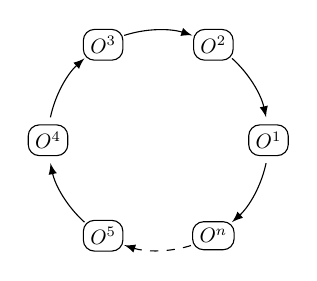
\begin{tikzpicture}[
circle/.style={
		scale=0.75,
		rounded corners,
		draw=black, 
		text centered,
		}
]

\def \n {6}
\def \m {4}
\def \radius {1.4cm}
\def \margin {12} % margin in angles, depends on the radius

\foreach \s in {1,...,\m}
{
  \node[draw, circle] at ({360/\n * (\s - 1)}:\radius) {$O^\s$};
  \draw[<-, >=latex] ({360/\n * (\s - 1)+\margin}:\radius) 
    arc ({360/\n * (\s - 1)+\margin}:{360/\n * (\s)-\margin}:\radius);
}

\node[draw, circle] at ({360/\n * 4}:\radius) {$O^5$};
  \draw[<-, dashed, >=latex] ({360/\n * 4+\margin}:\radius) 
    arc ({360/\n * 4+\margin}:{360/\n * (5)-\margin}:\radius);
    
\node[draw, circle] at ({360/\n * 5}:\radius) {$O^n$};
  \draw[<-, >=latex] ({360/\n * 5+\margin}:\radius) 
    arc ({360/\n * 5+\margin}:{360/\n * (6)-\margin}:\radius);


\end{tikzpicture}
\caption{Ring Settlement}
\label{fig:settlement}
\end{figurehere}
\end{center}

To make the transactions, the LPSC uses the \verb|TokenTransferDelegate| smart contract. The introduction of such a delegate makes upgrading the protocol smart contract easier as all orders only need to authorize this delegate instead of different versions of the protocol.

为了完成交易,路印协议智能合约使用了”代币传输委托智能合约”,引入这样一个委托使得协议智能合约升级更容易,因为所有的订单只需要授权这个委托而不是协议的不同版本。


For each order in the order-ring, a payment of \verb|tokenS| is made to the next or the previous order depending on the implementation. Then the ring-miner's fee is paid depending on the fee model chosen by the ring-miner. Finally, once all the transactions are made, a \verb|RingMined| event is emitted.

对于环路订单中的每一个订单,根据执行情况,代币的支付被分配给下一个订单或前一个订单。环路矿工费用取决于环路矿工选择的费用模型。最终,一旦所有交易全部完成,一次环路挖矿事件同时完成。


\subsubsection{发起事件\label{sec:events}}

The protocol emits events that allow relays, order browsers, and other actors to receive order book updates as efficiently as possible. The emitted events are:

协议发起的事件,允许中继,订单簿浏览器以及其他参与者尽可能高效率的接收最新的订单簿。这些发起的事件如下:


\begin{itemize}
	\item \textbf{OrderCancelled}: 一个指定的订单被取消

	\item \textbf{OrdersCancelled}: 一个地址对应某一个交易对的所有订单被取消
	\item \textbf{AllOrdersCancelled}: 一个地址对应的所有交易对的所有订单全部取消
	\item \textbf{RingMined}: 一个环路订单交易成功完成。这一事件包含了每一个内环代币传  
输数据
\end{itemize}


\section{LRx 代币\label{sec:token}}
LRx is our generalized token notation. LRC is the Loopring token on Ethereum, LRQ on Qtum, and LRN on NEO, etc. Other LRx types will be introduced in the future as Loopring is deployed on other public blockchains.

LRx是我们广义的代币符号。LRC是基于以太坊网络发行的路印协议代币,LRQ是基于量子链发行的路印协议代币,LRN是基于小蚁链发行的路印协议代币。随着路印协议在其他公有链上的部署,其他类型的路印协议代币LRx会随之发行。


\subsection{费用模型\label{sec:fee_model}} 
When a user creates an order, they specify an amount of LRx to be paid to the ring-miner as a fee, in conjunction with a percentage of the margin (\verb|marginSplitPercentage|) made on the order that the ring-miner can claim. This is called the margin split. The decision of which one to choose (fee or margin split) is left to the ring-miner.

当用户创建一个订单时,他们会指定一定数量的LRx作为支付给环路矿工的费用,结合环路矿工可以索取的边缘利润比例。这被称为边缘利润分割。由环路矿工决定选择用户指定的费用还是选择边缘利润分割作为矿工费用。


A representation of the margin split:

一个典型的利润分割如下:


\begin{center}
\begin{figurehere}
\centering
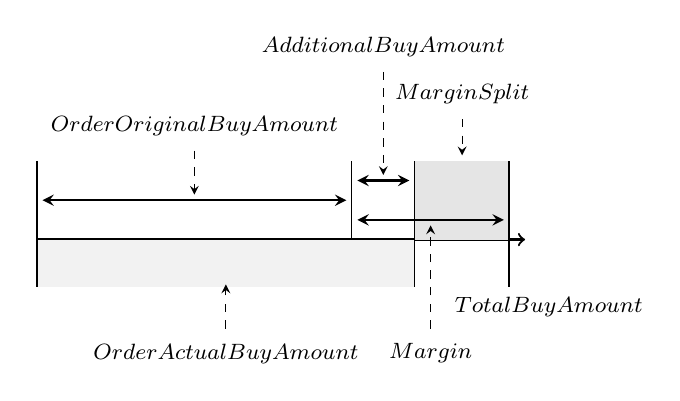
\begin{tikzpicture}[
scale=1,
font=\bfseries\footnotesize\sffamily,
classical/.style={thick,<->,shorten >=2pt,shorten <=2pt,>=stealth},
oneway/.style={->,dashed,shorten >=2pt,shorten <=2pt,>=stealth}
]
    % Draw axes
    \draw [->,thick] (0,1) node (yaxis) [above] {$$}
        |- (6.2,0) node (xaxis) [right] {$$};
        
    \draw
  	(4,0) coordinate (A)
  	(4,1) coordinate (A2)
  	(4.8,-0.6) coordinate (B)
  	(4.8,1) coordinate (B2)
  	(6,-0.6) coordinate (C)
  	(6,1) coordinate (C2);
  	
  	\fill [draw=none, fill=gray!20] 
    (4.8, 0) rectangle (6, 1);
    
  	\fill [draw=none, fill=gray!10] 
    (0, -0.6) rectangle (4.8, 0);

	\draw[thick] (0, -0.6) -- (0, 0.6) node[below]{$$};
  	\draw[thick, thin] (A) -- (A2) node[below]{$$};
  	\draw[thick, thin] (B) -- (B2) node[below]{$$};
  	\draw[thick] (C) node[below, xshift=0.5cm]{$Total Buy Amount$} -- (C2) ;
  	
  	\draw[classical] (0, 0.5) -> (4, 0.5) node[below]{$$};
  	\draw[classical] (4, 0.75) -> (4.8, 0.75) node[below]{$$};
%  	\draw[classical] (4.8, 0.5) -> (6, 0.5) node[below]{$$};
  	\draw[classical] (4, 0.25) -> (6, 0.25) node[below]{$$};

  	
  	\draw[oneway] (2, 1.2) node[above]{$Order Original Buy Amount$} -- (2, 0.5);
  	\draw[oneway] (4.4, 2.2) node[above]{$Additional Buy Amount$} -- (4.4, 0.75);
  	\draw[oneway] (5.4, 1.6) node[above]{$Margin Split$} -- (5.4, 1);
  	\draw[oneway] (5, -1.2) node[below]{$Margin$} -- (5, 0.25);
  	\draw[oneway] (2.4, -1.2) node[below]{$Order Actual Buy Amount$} -- (2.4, -0.5);



\end{tikzpicture}
\caption{A 60\% Margin Split}
\label{fig:marginsplit}
\end{figurehere}
\end{center}

If the margin on the order-ring is too small, a ring-miner will choose the LRx fee. If, on the contrary, the margin is substantial enough for the resulting margin split to be worth much more than the LRx fee, a ring-miner will choose the margin split. There is another proviso, however: when the ring-miner chooses the margin split, they must pay the user (order creator) a fee, which is equal to the LRx the user would have paid to the ring-miner as a fee. This increases the threshold of where the ring-miner will choose the margin split to twice the LRx fee of the order, increasing the propensity of the LRx fee choice. This allows ring-miners to receive a constant income on low margin order-rings for the tradeoff of receiving less income on higher margin order-rings. Our fee model is based on the expectation that as the market grows and matures, there will be fewer high margin order-rings, thus necessitating fixed LRx fees as incentive.

如果环路订单的边缘利润太少,环路矿工将会选择用户指定的LRx作为矿工费。相反,如果边缘利润数量足够多以至于边缘利润分割后分配到的价值比用户指定的LRx价值更高,那么环路矿工将会选择边缘利润分割。然而,还有另外一个条件,即当环路矿工选择边缘利润分割后,他们必须给用户支付订单创建费用,这个费用与用户指定的矿工费等价值。这提高了矿工选择边缘利润分割的门槛,增加了矿工选择用户指定的LRx作为矿工费的倾向,因为矿工从边缘利润分割获取的利润至少要双倍于用户指定的LRx。这使得在边缘利润较低的环路订单上获取的收入是比较稳定的。我们的费用模式的制定是基于一定的预期,即随着市场的成长与成熟,高边缘利润环路订单将会越来越少,因此需要固定的LRx费用作为激励。


We end up with the following graph:

我们以下图结束:


\begin{center}
\begin{figurehere}
\centering
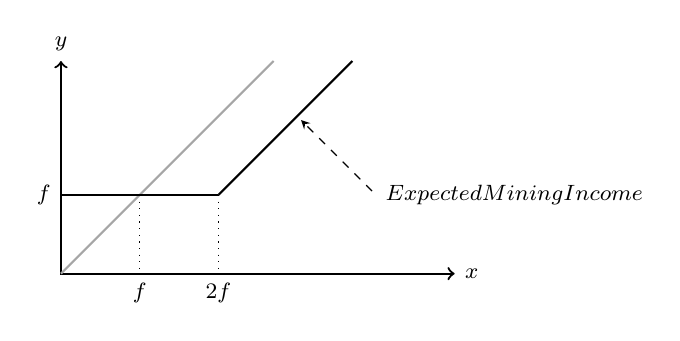
\begin{tikzpicture}[
font=\bfseries\footnotesize\sffamily,
oneway/.style={->,dashed,shorten >=2pt,shorten <=2pt,>=stealth},
scale=1]
    % Draw axes
    \draw [<->,thick] (0,2.7) node (yaxis) [above] {$y$}
        |- (5,0) node (xaxis) [right] {$x$};
        
    \draw
  	(1,1) coordinate (A)
  	(2,1) coordinate (B);
  	
  	
  	\draw[thick] (B) -- (3.7,2.7);
  	\draw[dotted] (B) -- (2,0) node[below] {$2f$};
  	\draw[dotted] (A) -- (1,0) node[below] {$f$};
  	\draw[thick,color=gray!70] (0,0) -- (2.7,2.7);
  	\draw[thick] (0,1) node[left] {$f$}--(B) node[     ]{$$};
 	\draw[oneway] (4,1) node[right]{$Expected Mining Income$} -- (3, 2);


\end{tikzpicture}
\caption{Loopring's Fee Model}
\label{fig:feemodel}
\end{figurehere}
\end{center}


where $f$ is the LRx fee, $x$ is the margin split, $y$ is the mining income. $y=max(f, x-f)$ as indicated by the solid line; if the LRx fee for the order is $0$, the equation is $y=max(0, x - 0)$ that simplifies to $y=x$ as indicated by the gray line.

f是费用LRx,x是边缘利润分割,y是挖矿收入。y=max(f, x-f) 如图中黑色实线所表示;如果订单的LRx费用是0,则y=max(0, x-0)简化为y=x如图中灰线所表示。



The consequences are:  

结果费用的选择如下:


\begin{enumerate}
	\item If the margin split is 0, ring-miners will choose the flat LRx fee and are still incentivized. 
	\item 如果边缘利润分割=0,环路矿工仍然会受到激励,矿工将会选择LRx作为矿工费用

	\item If the LRx fee is 0, the gray line results and the income is based on a general linear model.
	\item 如果费用LRx=0,结果由灰色线主导,此时收入基于线性模型计算。

	\item When the margin split income is greater than 2x(LRx fee), ring-miners choose the margin split and pay LRx to the user.
	\item 当边缘利润分割收入大于2*LRx费用,环路矿工将会选择边缘利润分割作为收入同时支付LRx给用户。

\end{enumerate}

It should be noted that if the LRx fee is non-zero, no matter which option the ring-miner chooses, there will always be a transfer of LRx between the ring-miner and the order's sender. Either the ring-miner earns the LRx fee, or pays the LRx fee back to the sender to take the margin split.

需要注意的是:如果LRx费用不等于0,那么不管环路矿工做了何种选择,在环路矿工与订单发送者之间都会有LRx的传输。要么是环路矿工赚取了LRx作为矿工费用,要么是环路矿工选择了边缘利润分割作为费用因而将LRx返还给订单发送者。


Ring-miners will share a certain percentage of fees with wallets. When a user places an order through a wallet and gets filled, the wallet is rewarded with a portion of the fees or margin split. Although this is modular, and unique business models or implementations are possible, our inclination is for wallets to receive approximately 20\%-25\% of earned fees. Wallets represent a primary target for Loopring protocol integration as they have the user base, but little or no source of income.

环路矿工会与钱包分享一定比例的费用。当用户通过钱包提交订单并且完成交易,作为奖励钱包将会收到部分费用或者部分边缘利润分割收入。尽管这是模块化的,独特的商业模式也是可以执行的,我们倾向于为钱包收取大约20\% ~ 25\%的费用。钱包代表了路印协议整合的初步目标,因为钱包拥有用户基础,但是钱包没有或者只有很少的收入来源。


\subsection{去中心化治理}
At its root, the Loopring protocol is a social protocol in the sense that it relies on coordination amongst members to operate effectively towards a goal. This is not dissimilar to cryptoeconomic protocols at large, and indeed, its usefulness is largely protected by the same mechanisms of coordination problems \cite{vitalikgovernance}, grim trigger equilibrium, and bounded rationality. To this end, LRx tokens are not only used to pay fees, but also to align the financial incentives of the various network participants. Such alignment is necessary for broad adoption of any protocol, but is particularly acute for exchange protocols, given that success rests largely on improving liquidity in a robust decentralized ecosystem.

从根本上来说,路印协议是一个社会协议,因为它依靠成员之间的相互协调,高效率的朝着一个目标前进。与一般的加密经济协议是不一样,事实上,它的效用在很大程度上受到同样的协调问题[20]、严格的触发平衡和有限理性的保护。为此目的,LRx代币不仅可以用来支付费用,也可以用来将各种网络参与者的经济激励达成一致。这种一致性对于广泛采用的任何协议都是必要的,但对于交换协议尤为重要,因为在一个强大的去中心化态系统中成功主要取决于流动性的改善。


LRx tokens will be used to effectuate protocol updates through decentralized governance. Smart contract updates will, in part, be governed by token holders to ensure continuity and safety, and to attenuate the risks of siphoned liquidity through incompatibility. Given that smart contracts cannot be altered once deployed, there is a risk that dApps or end users continue to interact with deprecated versions and preclude themselves from updated contracts. Upgradeability is crucial to the protocol's success as it must adapt to market demands and the underlying blockchains. Decentralized governance by LRx stakeholders will allow for protocol smart contract updates without disrupting dApps or end users, or relying too heavily on smart contract abstraction. LRx tokens have a fixed supply, and in the case of LRC, certain percentages are frozen from the Loopring Foundation, and allocated to community-purposed funds \cite{LRCtokendoc}.

However, LRx token owners are not the only stakeholders to consider in steering the protocol's direction: relays/ring-miners, wallets, developers, and others are an integral part of the ecosystem and their voice must be heard. In fact, given that these agents need not hold any LRx to perform their respective roles (since traditional makers/takers and market-makers are nonexistent, initial token reserves are not mandatory) we must allow alternative methods for their interests to be respected. Furthermore, "simple" token-based voting, both on-chain and off, is an imperfect salve for disagreement, as low voter turnout and token ownership concentration pose risks. Thus, the goal is to implement a governance model that is built in layers, and rests on a shared knowledge that some set of decision-making processes is the norm. This can be facilitated by coordination institutions that offer signals from a diverse set of participants, and, perhaps, from pre-established protocol focal points. As this comes to fruition, the Loopring Foundation will inevitably evolve from protocol developers into protocol stewards.

LRx代币将被用于通过去中心化的治理机制完成协议更新。智能合约的更新将由代币持有者管理以保证连续性和安全性,降低由兼容性引起的流动性降低的风险。考虑到智能合约一旦部署就不能更改,Dapp或终端用户继续使用过时的版本而且不更新合约是有风险的。对于协议的成功,升级能力是至关重要的,因为他必须满足市场需求以及底层区块链的需求。LRx代币持有人的去中心化治理模式允许在不扰乱Dapp或者终端用户的情况下进行协议智能合约更新。首先,这将通过一个简单的多重签名的智能合约完成,以期实现一种去中心化自治组织类型的机制。


\section{欺诈与攻击保护}

\subsection{防止抢先交易\label{sec:dual_authoring}}

In decentralized exchanges, front-running is when someone tries to copy another node's trade solution, and have it mined before the original transaction that is in the pending transaction pool (mempool). This can be achieved by specifying a higher transaction fee (gas price). The major scheme of front-running in Loopring (and any protocol for order-matching) are order-filch: when a front-runner steals one or more orders from a pending order-ring settlement transaction; and, specific to Loopring: when a front-runner steals the entire order-ring from a pending transaction.

在去中心化交易所中,抢先交易是指某人抄袭其他节点的交易解决方案,抢先于位于等待交易池中的原始订单完成挖矿。这可以通过设定一个更高的交易费用获得。路印中的抢先交易就是窃取订单:一个抢先交易者从一个悬挂的环路订单交易中窃取一个或者多个订单,具体到路印,指的是一个抢先交易者从一个悬挂的订单交易中窃取整个环路订单。


When a submitRing transaction is not confirmed and is still in the pending transaction pool, anyone can easily spot such a transaction and replace \verb|minerAddress| with their own address (the \verb|filcherAddress|), then they can re-sign the payload with \verb|filcherAddress| to replace the order-ring's signature. The fincher can set a higher gas price and submit a new transaction hoping block-miners will pick his new transaction into the next block instead of the original submitRing transaction.

当一个已提交的环路交易没有被确认并且仍然处于悬挂的交易池中时,任何人都可以很容易地发现这个交易,并用自己的地址(窃取者的地址)代替矿工地址,然后他们用窃取者的地址替换环路订单签名。偷盗者可以设置一个更高的费用并且提交一个新的交易,希望区块矿工能够将新的交易(而不是原始订单交易)写入下一个区块。


Previous solutions to this problem had important downsides: requiring more transactions and thus costing ring-miners more gas; and taking at least twice the blocks to settle an order-ring.  Our new solution, Dual Authoring\cite{dualauthor}, involves the mechanism of setting up two levels of authorization for orders - one for settlement, and one for ring-mining.

先前的针对这个问题的解决方案有很大的缺点:需要更多的交易并花费环路矿工更多的费用;至少需要花费双倍的费用才能完成一个环路订单。我们新的解决方案,双重授权涉及到了为订单进行两级授权的机制,一重授权是为了交易清算,另外一重授权用于环路挖矿。

Dual Authoring process:

双重授权过程如下:


\begin{enumerate}

	\item For each order, the wallet software will generate a random public-key/private-key pair, and put the key pair into the order's JSON snippet. (An alternative is to use the address derived from the public-key instead of the public-key itself to reduce byte size. We use \verb|authAddr| to represent such an address, and \verb|authKey| to represent \verb|authAddr|'s matching private-key).
	\item 对每一个订单,钱包软件会随机生成一个公钥/私钥对,公钥/私钥对将会被放入订单的JSON代码段中。(另一种方法是使用来自公钥的地址而不是公钥本身来减少字节大小,我们使用授权地址来代表这样一个地址,授权密钥代表授权地址匹配私钥。)


	\item Compute the order's hash with all fields in the order except \verb|r|, \verb|v|, \verb|s|, and \verb|authKey|), and sign the hash using the \verb|owner|'s private-key (not \verb|authKey|).
	\item 计算订单中除了r,v,s以及授权密钥以外所有字段的散列数值,并使用用户私钥进行签名(非授权密钥)。


	\item The wallet will send the order together with the \verb|authKey| to  relays for ring-mining. Ring-miners will verify that \verb|authKey| and \verb|authAddr| are correctly paired and the order's signature is valid with respect to \verb|owner| address.
	\item 钱包将订单与授权密钥一起发送给中继用于环路挖矿。环的矿工将验证授权密钥和授权地址正确配对,验证订单的签名对用户地址有效。


	\item When an order-ring is identified, the ring-miner will use each order's \verb|authKey| to sign the ring's hash, \verb|minerAddress|, and all the mining parameters. If an order-ring contains $n$ orders, there will be $n$ signatures by the $n$ \verb|authKey|s. We call these signatures the \verb|authSignature|s. The ring-miner may also need to sign the ring's hash together with all mining parameters using \verb|minerAddress|'s private-key.
	\item 当一个订单被验证有效时,环路矿工将会使用每一个订单的授权密钥为环路散列数值,矿工地址以及所有的挖矿参数进行签名。


	\item The ring-miner calls the submitRing function with all the parameters, as well as all the extra \verb|authSignature|s. Notice that \verb|authKey|s are NOT part of the on-chain transaction and thus remain unknown to parties other than the ring-miner itself.
	\item 如果一个环路订单包含了n个订单,将会有n个授权密钥进行n次签名。我们把这些签名称作授权签名。环路矿工也需要对环路哈希值进行签名,环形矿工可能还需要使用矿工地址私钥为环路哈希数值以及所有挖矿参数进行签名。


	\item The Loopring Protocol will now verify each \verb|authSignature| against the corresponding \verb|authAddr| of each order, and reject the order-ring if any \verb|authSignature| is missing or invalid.
	\item 路印协议将会验证与每一个订单的授权地址对应的授权签名,如果某个授权签名缺失或者无效,那么这个环路订单将会被拒绝。

 
\end{enumerate}

The result is that now:

结果如下:


\begin{itemize}

	\item  The order's signature (by the private-key of the \verb|owner| address) guarantees the order cannot be modified, including the \verb|authAddr|.
	\item 由用户地址的私钥完成的订单签名保证了订单以及授权地址无法串改。

	\item  The ring-miner's signature (by the private-key of the \verb|minerAddress|), if supplied, guarantees nobody can use his identity to mine an order-ring.
	\item 由矿工地址的私钥完成的环路矿工签名保证了没有人可以冒充它的身份进行环路挖矿。

	\item  The \verb|authSignature|s guarantees the entire order-ring cannot be modified, including \verb|minerAddress|, and no orders can be stolen.
	\item 授权签名保证了整个环路订单以及矿工地址无法被串改,没有订单会被窃取。


\end{itemize}

Dual Authoring prevents ring-filch and order-filch while still ensuring the settlement of order-rings can be done in one single transaction. In addition, Dual Authoring opens doors for relays to share orders in two ways: non-matchable sharing and matchable sharing. By default, Loopring operates an OTC model and only supports limit-price orders, meaning that orders' timestamps are ignored. This implies that front-running a trade has no impact on the actual price of that trade, but does impact whether it gets executed or not.

双重授权防止了环路窃取与订单窃取,但仍然能够保证环路订单可以在一个交易中完成。此外,双重授权以两种方式为中继共享订单打开了大门:对等共享与非对等共享。默认情况下,路印支持场外交易模型并且只支持限价订单,这意味着订单的时间戳被忽略。这就意味或着抢先交易对实际交易的价格没有影响,但是订单是否可以执行会受到影响。


\section{其他攻击}

\subsection{Sybil or DOS 攻击}
Malicious users -- acting as themselves or forged identities -- could send a large amount of small orders to attack Loopring nodes. However, since we allow nodes to reject orders based on their own criteria -- which they may hide or reveal -- most of these orders will be rejected for not yielding satisfying profit when matched.  By empowering relays to dictate how they manage orders, we do not see a massive tiny order attack as a threat.

恶意用户可以以自己的身份或者伪造身份,发送大量的小订单攻击路印节点。但是,由于我们允许节点根据自己的标准(标准可以公开或者不公开)拒绝订单,大部分恶意订单在订单匹配时因得不到满意的利润而被拒绝。通过授权中继来控制如何管理订单,我们不认为大规模的小订单攻击会产生威胁。


\subsection{资产余额不足}
Malicious users could sign and spread orders whose order value is non-zero but whose address actually has zero balance. Nodes could monitor and notice that some orders actual balance is zero, update these order states accordingly and then discard them.
Nodes must spend time to update the status of an order, but can also choose to minimize the effort by, for example, blacklisting addresses and dropping related orders.

恶意用户可以签署并传播订单值不为0的订单,但是这些地址实际上资产为0。节点可以监控并注意到某些订单实际上资产余额为0,相应的更新这些订单状态并丢弃这些订单。节点必须花费事件更新订单状态,但是可以通过黑名单地址并放弃与之相关的订单来减少工作量。


\section{总结}

The Loopring protocol sets out to be a foundational layer for decentralized exchange. In so doing, it has profound repurcussions in how people exchange assets and value. Money, as an intermediate commodity, facilitates or replaces barter exchange and solves the double coincidence of wants problem \cite{unenumerated2006}, whereby two counterparties must desire each other's distinct good or service. Similarly, Loopring protocol aims to dispense of our dependencies on coincidence of wants in trading pairs, by using ring matching to more easily consummate trades. This is meaningful for how society and markets exchange tokens, traditional assets, and beyond. Indeed, just as decentralized cryptocurrencies pose threat to a nation's control over money, a combinatorial protocol that can match traders (consumers/producers) at scale, is a theoretical threat to the concept of money itself.

路印协议被设置为去中心化交易所的基础层。这样做对人们如何交换资产与价值产生了深刻的影响。作为一种中间商品,货币有助于替代物物交易解决了双重需求偶合问题[22],双重需求偶合指两个交易对手必须相互需求对方的物品或服务。类似的,路印协议通过环路匹配更容易完成交易,路印协议旨在消除对交易对双重需求偶合的依赖。这对于社会和市场交易代币,传统资产,以及其他方面意义重大。事实上,正如去中心化加密货币对一个国家货币体系造成的威胁,可以规模化匹配订单的组合协议理论上对货币概念本身也是一种威胁。

Protocol benefits include:

协议的好处包括:

\begin{itemize}
	\item Off-chain order management and on-chain settlement means no sacrifice in performance for security.
	\item 链下管理订单链上完成订单意味着并没有牺牲性能与安全性。

	\item Greater liquidity due to ring-mining and order sharing.
	\item 环路挖矿与订单共享带来巨大的流动性。

	\item Dual Authoring solves the pernicious problem of front running faced by all DEXs and their users today.
	\item 双重授权解决了所有去中心化交易所与用户面临的抢先交易问题。

	\item Free, public smart contracts enable any dApp to build or interact with the protocol.
	\item 任何Dapp都可以内嵌免费公开的智能合约,并与协议相互通信。

	\item Standardization among operators allows for network effects and an improved end user experience.
	\item 运营商之间的标准化提升了网络效应和改进了终端用户体验。

	\item Network maintained with flexibility in running order books and communicating.
	\item 订单运行与通信灵活,网络维护具有弹性。

	\item Reduced barriers to entry means lower costs for nodes joining the network and end users.
	\item 降低参与壁垒意味着节点加入网络与终端用户的费用更低。

	\item Anonymous trading directly from user wallets.
	\item 直接通过用户钱包进行匿名交易。

\end{itemize}

\section{致谢}
We would like to express our gratitude to our mentors, advisers and to the many people in the community that have been so welcoming and generous with their knowledge. In particular, we would like to thank Shuo Bai (from ChinaLedger); Professor Haibin Kan; Alex Cheng, Hongfei Da; Yin Cao; Xiaochuan Wu; Zhen Wang, Wei Yu, Nian Duan, Jun Xiao, Jiang Qian, Jiangxu Xiang, Yipeng Guo, Dahai Li, Kelvin Long, Huaxia Xia, Jun Ma, and Encephalo Path for reviewing and providing feedback on this project. 

谨向我们的导师、顾问和社区中的许多人表示感谢,向他们渊博的学识表示敬意。特别感谢中国分布式总账基础协议联盟ChinaLedger的白硕;阚海滨教授;Alex Cheng,达鸿飞;曹寅;吴晓川;王震;于伟;段念;小俊;钱江;向江旭;郭一鹏;李大海;Kelvin Long;夏华夏;马俊;以及Encephalo Path对项目的审查与意见反馈。


\bibliography{whitepaper}
\bibliographystyle{unsrt}


\end{multicols}


\begin{appendices}

\section{Loopring on Ethereum\label{app:protocol_ethereum}}

\subsection{Smart Contracts}

\begin{center}
\begin{figurehere}
\centering
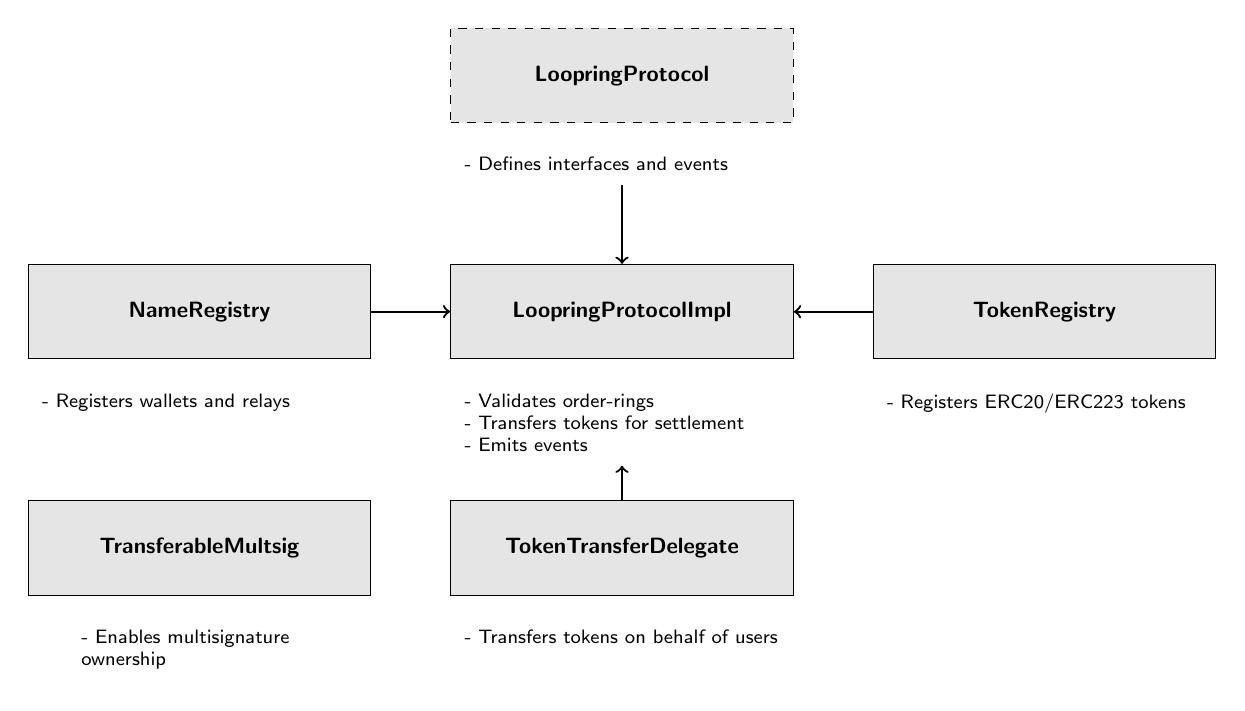
\begin{tikzpicture}
[node distance = 1cm, auto,font=\footnotesize,
% STYLES
every node/.style={node distance=3cm},
% The comment style is used to describe the characteristics of each force
comment/.style={rectangle, inner sep= 5pt, text width=4cm, node distance=0.25cm, font=\scriptsize\sffamily},
% The force style is used to draw the forces' name
force/.style={rectangle, draw, fill=black!10, inner sep=5pt, text width=4cm, text badly centered, minimum height=1.2cm, font=\bfseries\footnotesize\sffamily}] 

% Draw forces
\node [force] (impl) {LoopringProtocolImpl};
\node [force, dashed, above of=impl] (protocol_interface) {LoopringProtocol};
\node [force, left=1cm of impl] (nameregistry) {NameRegistry};
\node [force, right=1cm of impl] (tokenregistry) {TokenRegistry};
\node [force, below of=impl] (delegate) {TokenTransferDelegate};
\node [force, left=1cm of delegate] (multisig) {TransferableMultsig};

%%%%%%%%%%%%%%%
% Change data from here

% impl
\node [comment, below=0.25 of impl] (comment-impl) {- Validates order-rings\\
- Transfers tokens for settlement\\
- Emits events};

% nameregistry
\node [comment, below=0.25cm of nameregistry]{- Registers wallets and relays};

% protocol_interface
\node [comment, below=0.25 of protocol_interface](comment-interface) {- Defines interfaces and events};

% tokenregistry
\node [comment, below=0.25 of tokenregistry] {- Registers ERC20/ERC223 tokens};

% delegate
\node [comment, below=0.25 of delegate] {- Transfers tokens on behalf of users};

% PUBLIC POLICIES
\node [comment, text width=3cm, below=0.25 of multisig] {- Enables multisignature ownership};

%%%%%%%%%%%%%%%%

% Draw the links between forces
\path[->,thick] 
(comment-interface) edge (impl)
(nameregistry) edge (impl)
(tokenregistry) edge (impl)
(delegate) edge (comment-impl);

\end{tikzpicture} 
\caption{Smart Contracts}
\label{fig:smartcontracts}
\end{figurehere}
\end{center}

\subsection{Deployment}

The following smart contracts have been deployed on Ethereum mainnet:
\begin{itemize}
\item LRC: \verb|0xEF68e7C694F40c8202821eDF525dE3782458639f|
\item TokenRegistry: \verb|0xa21c1f2AE7f721aE77b1204A4f0811c642638da9|
\item TokenTransferDelegate: \verb|0xc787aE8D6560FB77B82F42CED8eD39f94961e304|
\item NameRegistry: \verb|0x0f3Dce8560a6010DE119396af005552B7983b7e7|
\item LoopringProtocolImpl: \verb|0xc80BbAb86cED62CF795619A357581FaF0cB46511|
\item TransferableMultsig: \verb|0x7421ad9C880eDF007a122f119AD12dEd5f7C123B|
\end{itemize}

\end{appendices}
\end{document}
